%%
%% This is file `sample-acmsmall.tex',
%% generated with the docstrip utility.
%%
%% The original source files were:
%%
%% samples.dtx  (with options: `acmsmall')
%% 
%% IMPORTANT NOTICE:
%% 
%% For the copyright see the source file.
%% 
%% Any modified versions of this file must be renamed
%% with new filenames distinct from sample-acmsmall.tex.
%% 
%% For distribution of the original source see the terms
%% for copying and modification in the file samples.dtx.
%% 
%% This generated file may be distributed as long as the
%% original source files, as listed above, are part of the
%% same distribution. (The sources need not necessarily be
%% in the same archive or directory.)
%%
%% The first command in your LaTeX source must be the \documentclass command.
\documentclass[acmsmall]{acmart}

%%
%% \BibTeX command to typeset BibTeX logo in the docs
\AtBeginDocument{%
  \providecommand\BibTeX{{%
    \normalfont B\kern-0.5em{\scshape i\kern-0.25em b}\kern-0.8em\TeX}}}

\settopmatter{printacmref=false} % Removes citation information below abstract
\setcopyright{none}
\renewcommand\footnotetextcopyrightpermission[1]{} % removes footnote with conference information in first column
%\pagestyle{plain}

%% Rights management information.  This information is sent to you
%% when you complete the rights form.  These commands have SAMPLE
%% values in them; it is your responsibility as an author to replace
%% the commands and values with those provided to you when you
%% complete the rights form.
%\setcopyright{acmcopyright}
%\copyrightyear{2018}
%\acmYear{2018}
%\acmDOI{10.1145/1122445.1122456}


%%
%% These commands are for a JOURNAL article.
%\acmJournal{JACM}
%\acmVolume{37}
%\acmNumber{4}
%\acmArticle{111}
%\acmMonth{8}

%%
%% Submission ID.
%% Use this when submitting an article to a sponsored event. You'll
%% receive a unique submission ID from the organizers
%% of the event, and this ID should be used as the parameter to this command.
%%\acmSubmissionID{123-A56-BU3}

%%
%% The majority of ACM publications use numbered citations and
%% references.  The command \citestyle{authoryear} switches to the
%% "author year" style.
%%
%% If you are preparing content for an event
%% sponsored by ACM SIGGRAPH, you must use the "author year" style of
%% citations and references.
%% Uncommenting
%% the next command will enable that style.
%%\citestyle{acmauthoryear}
\usepackage{listings}
\usepackage{color}

\definecolor{dkgreen}{rgb}{0,0.6,0}
\definecolor{gray}{rgb}{0.5,0.5,0.5}
\definecolor{mauve}{rgb}{0.58,0,0.82}
\lstset{frame=tb,
	language=Java,
	aboveskip=3mm,
	belowskip=3mm,
	showstringspaces=false,
	columns=flexible,
	basicstyle={\small\ttfamily},
	numbers=none,
	numberstyle=\tiny\color{gray},
	keywordstyle=\color{blue},
	commentstyle=\color{dkgreen},
	stringstyle=\color{mauve},
	breaklines=true,
	breakatwhitespace=true,
	tabsize=3
}

\usepackage{subfigure}
\usepackage{lipsum}

%%
%% end of the preamble, start of the body of the document source.
\begin{document}

%%
%% The "title" command has an optional parameter,
%% allowing the author to define a "short title" to be used in page headers.
\title{Code Deobfuscation using Neural Program Learning Models}

%%
%% The "author" command and its associated commands are used to define
%% the authors and their affiliations.
%% Of note is the shared affiliation of the first two authors, and the
%% "authornote" and "authornotemark" commands
%% used to denote shared contribution to the research.
\author{Amin Fallahi}
\affiliation{%
	\institution{Syracuse University}
	\streetaddress{Center for Science and Technology, 111 College Pl}
	\city{Syracuse}
	\state{New York}
	%\country{USA}
}

%%
%% By default, the full list of authors will be used in the page
%% headers. Often, this list is too long, and will overlap
%% other information printed in the page headers. This command allows
%% the author to define a more concise list
%% of authors' names for this purpose.
\renewcommand{\shortauthors}{Fallahi, et al.}

%%
%% The abstract is a short summary of the work to be presented in the
%% article.
\begin{abstract}
	Code deobfuscation has gained attention in research for its wide applicability in forgery detection, privacy, and security. Several approaches have been proposed in past research that focus on identifier name recovery from a minified code or extracting information from obfuscated code, most of which use statistical or classical machine learning approaches to deobfuscate code and achieve notable performance. In this research, we study neural networks, specifically neural program learning models on this task. We focus on Neural Turing Machine as a model that has been proven to work well on remembering information using its memory. We build the network using NTM, prepare an existing data set, and evaluate the network with various parameters against the data set. Our evaluation results indicate that we get an average accuracy of around 60\% for most settings but under limited scenarios. However, there are possible improvements to this work that we leave for future research.
\end{abstract}

%%
%% The code below is generated by the tool at http://dl.acm.org/ccs.cfm.
%% Please copy and paste the code instead of the example below.
%%
%\begin{CCSXML}
%<ccs2012>
% <concept>
%  <concept_id>10010520.10010553.10010562</concept_id>
%  <concept_desc>Computer systems organization~Embedded systems</concept_desc>
%  <concept_significance>500</concept_significance>
% </concept>
% <concept>
%  <concept_id>10010520.10010575.10010755</concept_id>
%  <concept_desc>Computer systems organization~Redundancy</concept_desc>
%  <concept_significance>300</concept_significance>
% </concept>
% <concept>
%  <concept_id>10010520.10010553.10010554</concept_id>
%  <concept_desc>Computer systems organization~Robotics</concept_desc>
%  <concept_significance>100</concept_significance>
% </concept>
% <concept>
%  <concept_id>10003033.10003083.10003095</concept_id>
%  <concept_desc>Networks~Network reliability</concept_desc>
%  <concept_significance>100</concept_significance>
% </concept>
%</ccs2012>
%\end{CCSXML}
%
%\ccsdesc[500]{Computer systems organization~Embedded systems}
%\ccsdesc[300]{Computer systems organization~Redundancy}
%\ccsdesc{Computer systems organization~Robotics}
%\ccsdesc[100]{Networks~Network reliability}

%%
%% Keywords. The author(s) should pick words that accurately describe
%% the work being presented. Separate the keywords with commas.
\keywords{neural program learning, code deobfuscation, neural Turing machine}


%%
%% This command processes the author and affiliation and title
%% information and builds the first part of the formatted document.
\maketitle

\section{Introduction}
One of the trending methods for improving software security and hiding program codes from users is code obfuscation. Some codes are meant to run on the browsers and are widely used to create dynamic content in web-pages. Many service providers try to hide the code from the user to improve their security and obscure the real function of code. Using a simple obfuscation technique, the providers make their program secure against attackers but they are also able to inject malicious code that can help advertisement, tracking the user, collecting user information, cross-site scripting attacks, etc. Obfuscation targets changing the code in a way that makes it hard for the human to understand what the code is actually doing by methods like changing variable/function names, altering execution order, loop unrolling, character encoding, etc. In contrast, code deobfuscation methods try to gain as much information from obfuscated codes and extract the program from unreadable code.

%Past research on code deobfuscation has achieved good accuracy for identifier recovery. But to our knowledge, 
Using a Neural Program Learning (NPL) model for solving this problem and how it performs can be an interesting study. NPL models use neural networks which are trained to learn and replicate code behavior, produce code from input/outputs, or complete previously written code. Code deobfuscation is an application that can be extended to a program learning task. Specifically, we can treat obfuscated identifier names as unknown holes in a program code and try to recover them using an NPL algorithm.

In this research, we use neural program learning methods to recover identifier (variables and functions) names from obfuscated program code. We study some currently used obfuscation and deobfuscation methods and how much identifier names the current approaches to deobfuscation can recover. Then, we use Neural Turing Machine (NTM) \cite{ntm} as our program learning model and train it using publicly available data sets. Finally, we evaluate our work and try to optimize the network by altering and tuning parameters to improve the performance.

The main contributions of this work are:
\begin{itemize}
	\item Novel application of neural program learning models on code deobfuscation task.
	\item Preparing a neural activation dataset usable in neural networks based on publicly available program code datasets.
	\item Evaluating our neural program learning model and comparing it with the results of previous research for this task.
	\item Extending an existing Neural Turing Machine implementation to work with our model\footnote[1]{https://github.com/aminfallahi/Code-Deobfuscation-using-NTM}.
\end{itemize}

\textbf{Outline} In the remainder of this report, we introduce some of the related work that have been done in this research area in section 2. Then, we discuss basic background knowledge and area literature required for studying this work in section 3. In Section 4 we introduce the dataset we are using for this study and the preparation methods we use for making the data fit our model. Afterwards, we review the implementation details for Neural Turing Machine, our tweaks, and modifications to it for using with our application. We run our implementation through multiple experiments and present the results in section 6 and then we discuss the results and outcome of the research in section 7. In section 8 we discuss some possible extensions to this work which is left for future research and finally, we conclude the study in section 9.

\section{Related Work}
Research on code deobfuscation has been a topic of interest during the recent years. Jiang et al. \cite{jiangcnn} have proposed a method using Convolutional Neural Networks for detecting obfuscated JavaScript code. Raychev et al. \cite{jsnice1} have developed a statistical model for recovering program properties (variable and function names) from obfuscated JavaScript code  and have implemented a currently available website named JSNice \cite{jsnice3} which can predict the correct names for 63\% of identifiers from obfuscated code for their test data. They also have designed Nice2Predict \cite{nice2predict} which extracts statistical info out of obfuscated JavaScript code and is a base for JSNice. Raychev et al. \cite{Raychev2014} have done research on code completion and program synthesis which is relevant to our problem. Bichsel et. al. \cite{bichselandroid} have developed and tested a statistical method for deobfuscating Android applications with 79.1\% success in recovering program identifier names. Another relevant research is \cite{forth} which studies filling program missing code slots using the behavior trained from the program input/output data. Lin et al. \cite{nlprnn} have done relevant research on translating natural language templates to program templates using Recurrent Neural Networks.

\section{Background}
\subsection{Neural Program Learning}
Neural program learning is the use of program behavior to train deep neural networks so they perform like the program or produce the code based on input/outputs, partial programs, etc. So, a neural network can be used as a programmer and also an interpreter. The research in this area has been developed by several researchers during the past decade, varying from implementing logical gates using neural networks \cite{neto} to completing a partial program code \cite{forth}.
\subsection{Code Deobfuscation}
Obfuscation is a method used by programmers, specially in web services, to hide the running code from the user. When users visit a website using a browser with JavaScript enabled, several scripts will be executed in their browsers. The service providers, usually make the code unreadable by changing identifier names to meaningless tokens and then remove white space and tabs to decrease code size. Shrinking code size leads to less data transfer and faster page loading but changing identifier names is meant to hide the actual function of code from the user. Websites practice advertising, tracking, and other acts that are privacy concerns using these codes and hide the actual operation of the code by obfuscating it.

Several methods have been proposed for deobfuscation. Basic methods recover tabs and spaces to make the code more readable but are not capable of recovering the actual code including identifier names. Some methods use machine learning and statistical approaches to recover identifier names. Also, some approaches target deciphering code that has been encrypted using cryptography algorithms.

Listing 1. shows a piece of obfuscated JavaScript code grabbed from Facebook.com. This code is unminified using an online tool, Unminify \cite{unminify}, which inserts tabs and spaces for it to look more readable, but the identifier names will remain obfuscated. As we can see, most of them have been changed to single letter names, making it hard for anyone to understand what the code is actually doing.

Listing 2. shows the same code from Listing 1. deobfuscated using JSNice \cite{jsnice3} tool which uses statistical methods to recover identifier names. As we can see, some of the names have been recovered and the code is more understandable. However, we can not be sure how accurate are the names that are assigned to obfuscated identifiers.

\begin{lstlisting}[language=Java,caption={An obfuscated JavaScript code from facebook.com}]
__d("ContextualLayerAlignmentEnum", ["prop-types"], (function(a, b, c, d, e, f) {
	"use strict";
	a = {
		left: "left",
		center: "center",
		right: "right",
		propType: b("prop-types").oneOf(["left", "center", "right"]),
		values: ["left", "center", "right"]
	};
	e.exports = a
}), null);
\end{lstlisting}

\begin{lstlisting}[language=Java,caption={Deobfuscated JavaScript code from Listing 1. using JsNice\cite{jsnice} tool}]
'use strict';
__d("ContextualLayerAlignmentEnum", ["prop-types"], function(h, require, canCreateDiscussions, isSlidingUp, module, dontForceConstraints) {
	h = {
		left : "left",
		center : "center",
		right : "right",
		propType : require("prop-types").oneOf(["left", "center", "right"]),
		values : ["left", "center", "right"]
	};
	/** @type {(Object|string)} */
	module.exports = h;
}, null);
\end{lstlisting}




\subsection{Neural Turing Machine}
The idea behind Neural Turing Machines is to use an external memory to extend the capabilities of recurrent neural networks. The external memory and the network can then interact with attentional processes \cite{ntm,ntm1,ntm2}.

As shown in Fig. \ref{fig:ntmarch}, NTM is composed of two main components: the network controller and a memory bank which is basically a matrix used to store and retrieve information. In each time step, the network gets an input and produces an output. But NTM is also capable to perform read and write operations and alter the memory matrix. Like traditional Turing machines, NTM uses the term "head" to refer to a specific memory location \cite{ntm,ntm1,ntm2}.

\begin{figure}[h]
	\centering
	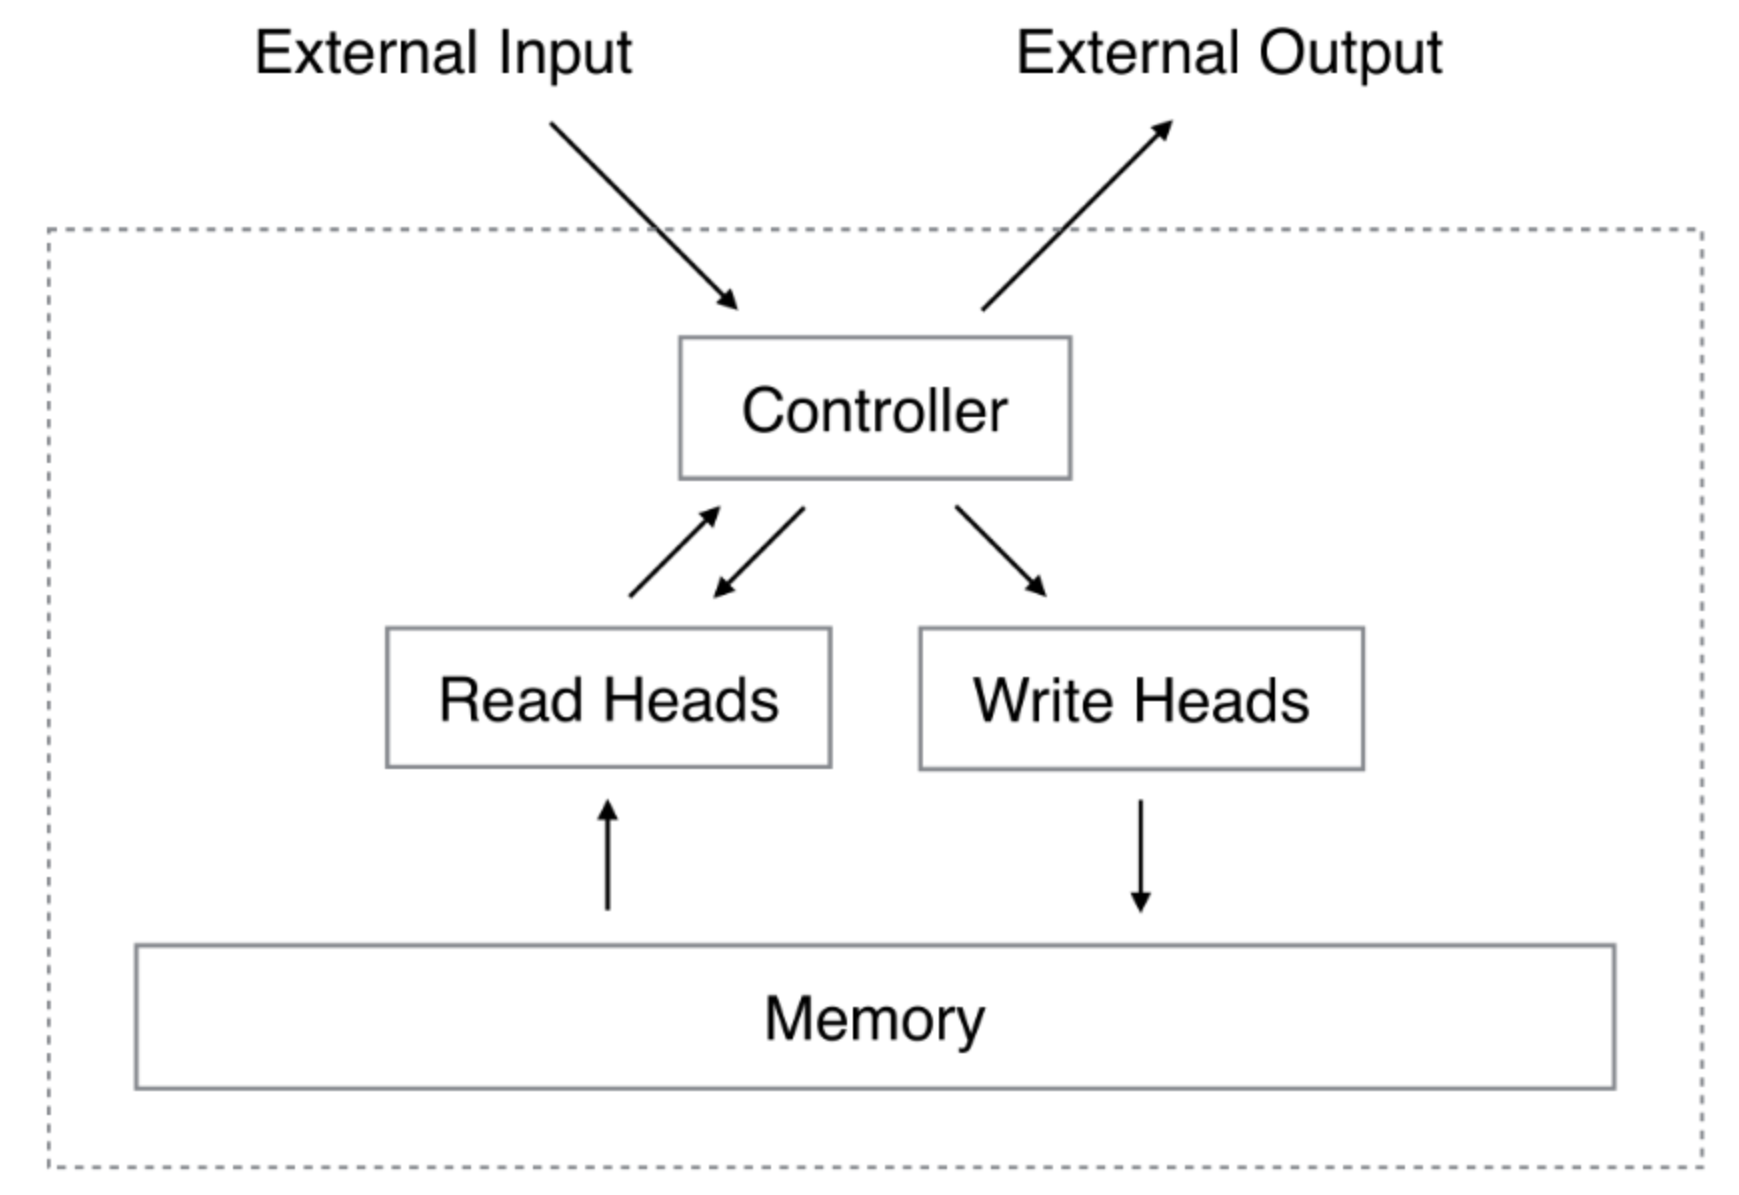
\includegraphics[scale=0.15]{figures/ntmarch}
	\caption{Neural Turing Machine architecture \cite{ntm}.}
	\Description{Neural Turing Machine architecture \cite{}.}
	\label{fig:ntmarch}
\end{figure}

For network training, it is preferred to use backpropagation and an optimizer like stochastic gradient decent (SGD) or Adam. For this purpose, NTM controller uses "blurry" reads and writes to interact with the memory, leading to the network being differentiable. That means, the controller uses a greater or lesser degree to read the whole memory instead of addressing and accessing each single element in memory. This is possible using an attention vector to focus on a part of memory and ignore the rest \cite{ntm,ntm1,ntm2}.

\subsubsection{Memory}
A memory $M_{t}$ is a $N \times M$ two dimensional matrix at time $t$, where $N$ indicates the number of memory locations, each storing a vector of size $M$.

\subsubsection{Read}
NTM uses a weighted sum of the memory for reading, where $w_t$ is a weight vector of size $N$ at time $t$:
\begin{equation}
r_t \longleftarrow \sum_{i} w_t(i)M_t(i)
\end{equation}

\subsubsection{Write}
A write operation is composed of an erase and an add operation. A vector $e_t$ of size $N$ is used for erasing and another vector $a_t$ is used for the add operation. Let $\tilde{M}_t$ be the intermediate memory after erase operation on $M_{t-1}$ and $1$ be a vector of ones:
\begin{equation}
\tilde{M_t}(i) \longleftarrow M_{t-1}(i)[1-w_t(i)e_t]
\end{equation}
Then, if both $w_t$ and $e_t$ at location $i$ are one, the memory location will reset to zero and if both are zero the memory will not be touched.

Finally, the add vector $a_t$ is used to perform the add operation on the intermediate memory state and produce the final memory matrix:
\begin{equation}
M_t(i) \longleftarrow \tilde{M}_t(i)+w_t(i)a_t
\end{equation}

\subsubsection{Addressing}
NTM produces the weighting vectors for read and write operations by combining content-based and location-based addressing mechanisms.

The content-based addressing compares a key vector $k_t$ with each $M_t(i)$ vector using cosine similarity (Equation 5) measure and produces a normalized weight vector $w_t^c$ based on the similarity and a key strength vector $\beta_t$ which is used for increasing or decreasing focus precision:
\begin{equation}
w_t^c(i) \longleftarrow {{exp(\beta_t K[k_t, M_t(i)])} \over {\sum_{j} exp(\beta_t K[k_t,M_t(j)])}}
\end{equation}
\begin{equation}
K[u,v] = {{u.v} \over {||u||.||v||}}
\end{equation}

For location-based addressing, a scalar parameter $g_t \in (0,1)$ is introduced which is called interpolation gate and is used to mix $w_t^c$ and $w_{t-1}$ to produce the gated weighting $w_t^g$. This lets the controller know when to use which kind of memory addressing:
\begin{equation}
w_t^g \longleftarrow g_t w_t^c + (1-g_t)w_{t-1}
\end{equation}

NTM controller uses circular convolutional shift with all index arithmetic computed modulo $N$ with a shift vector $s_t$ to change the focus to another memory location and produce the shifted weight vector $\tilde{w}_t(i)$:
\begin{equation}
\tilde{w}_t(i) \longleftarrow \sum_{j=0}^{N-1} w_t^g(j)s_t(i-j)
\end{equation}

Finally, a scalar $\gamma$ is used for sharpening the final weighting and preventing it from blurring:
\begin{equation}
w_t(i) \longleftarrow {\tilde{w}_t(i)^{\gamma_t}} \over {\sum_{j} \tilde{w}_t(j)^{\gamma_t}}
\end{equation}

Figure \ref{fig:ntmaddressing} shows the flow of addressing mechanism \cite{ntm,ntm1,ntm2}.

\begin{figure}[h]
	\centering
	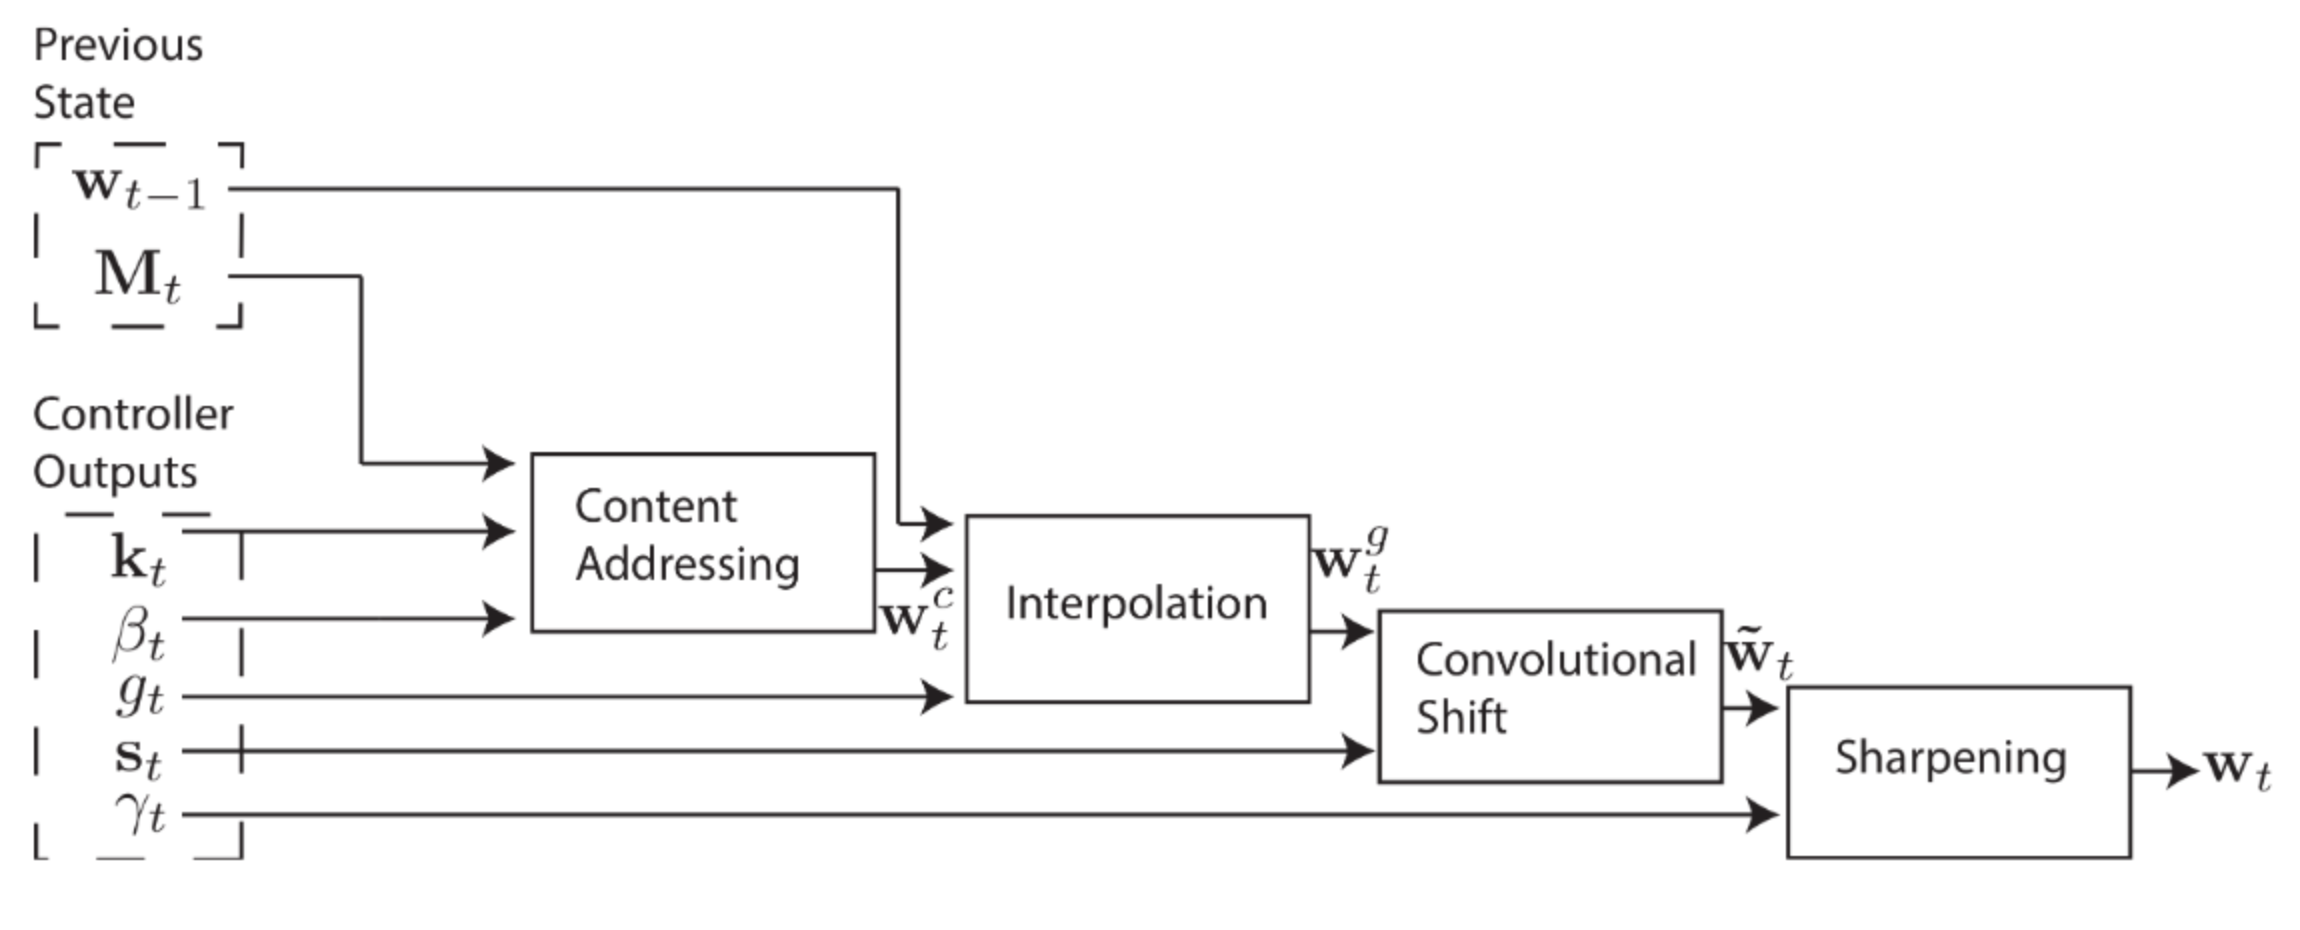
\includegraphics[scale=0.15]{figures/ntmaddressing}
	\caption{Flow diagram of Neural Turing Machine addressing mechanism \cite{ntm}.}
	\Description{Flow diagram of Neural Turing Machine addressing mechanism \cite{ntm}.}
	\label{fig:ntmaddressing}
\end{figure}

\section{Dataset Preparation}
Researchers in Secure, Reliable, and Intelligent Systems Lab \cite{srilab} at ETH Zurich have collected and published a data set of 150000 JavaScript programs and 150000 Python scripts as a part of their research \cite{jsnice2} which is publicly available at \cite{bigcodedataset}. They also have parsed the programs and generated abstract syntax trees (AST) for all the programs in json format. In this research, we build our dataset on top of their raw Python code dataset. For simplicity, we filter a set of 1848 programs each with less than 20 lines of code and smaller than 1 Kilobyte and truncate codes with unicode and non-ascii characters. Then, we use a simple Python tokenizer \cite{tokenizer} to extract all the tokens used in all programs. We sort the tokens and remove duplicates to create our final list containing 22973 tokens addressable with 15 binary bits. Afterwards, we create a list of vectors starting from 0b000000000000000 to 0b101100110111101 (22973) each representing one token. Finally, we use pyminify \cite{pyminify} (which is a simple tool for minifying Python codes) with --rename-globals option to rename all the variables to generate our obfuscated dataset and then we convert each program to a set of vectors based on their tokens and store the resulting dataset.

\section{Implementation}
The original authors of Neural Turing Machine have not published their source code to the public, but since 2014, multiple open source implementations have been released by various groups. Most of the implementations are limited and unstable. One of the recent implementations which is more robust and reliable is the one by Collier et al. \cite{collier} which has won a best paper award. Therefore, we chose to modify their code to fit our application and use it for this research.

This implementation uses LSTM (Long Short-Term Memory) \cite{lstm} as the controller of the NTM and evaluates the model with three tasks: copy task that generates the same output by copying the input; repeat-copy task that extends copy task to copying input for specific number of times and producing it as output; associative recall that feeds a list of items to the network, queries one of them, and expects the next item in the list to be produced in output \cite{ntm1}.

We modify copy task for our application. However, our data inputs and outputs are different, so we are not using it for copying the input to output.

This implementation uses random sequences of vectors as data. We implement a new data generator function to use our dataset instead of the randomly generated one. For our dataset to fit the NTM implementation, we write a program to generate data batches. As an example for one configuration, each input sequence stores 128 token vectors and one vector of all ones indicating the end of sequence. The rest of sequence will be padded to 257 (2 times number of tokens minus 1 for the termination vector) vectors using vectors of all zeros. We also add one zero to all token vectors except the termination vector to differentiate them from it. So, the final shape of each input will be 257x16 where 16 is the batch size. Each output sequence stores 128 token vectors of 15 bits resulting in a shape of 128x15. The final batch that fits the NTM implementation we use is in the $[(sequence_length, array([[[]]], dtype=float32))]$ format and stores sequence length (128) and $n$ batches of inputs and outputs.

We continue our modification by introducing perturbation functions. The goal is to add noise and shuffle data to evaluate the effect of them on the results later. We add three parameters to the program: whether to shuffle the tokens in input and accordingly in output, percent of noise to be added to the token sequences, and percent of noise to be added to each batch of inputs. For shuffling the input and output sequences, we generate a permutation of 128 integers by shuffling the range of integers between 0 to 127. Then, we sort the tokens based on the permutation both in input and output. For adding noise to the input sequence, we use a shuffled range list again and choose first $n$ integers from the shuffled list based on the percentage of noise we want to add. Then, we replace the randomly chosen token vectors with random vectors of 0 and 1. We do the same procedure for creating a random matrix of 0 and 1 and replace the indicated percent of generated input programs with random matrices.

\section{Evaluation}
We evaluate our model in different scenarios, each changing one parameter of the network architecture or a parameter of input/output data. In all experiments, we use 500 training steps. However, an NTM takes many more training steps to produce notable results and it would take a long time for each training procedure which does not fit our limited time for evaluating the model under multiple scenarios. We use gradient decent with Adam optimizer for training our network with 1000 program codes. Then, 848 programs will be left from our dataset that we use as testing data.

We discuss our experiments in the remainder of this section and present our results in Fig. \ref{fig:training} and Fig. \ref{fig:testing}. The former shows training performance for 500 sequences and the latter compares testing performance under fixed size dataset and variable sized dataset for 500 testing sequences. We aggregate our data in Fig. \ref{fig:testing} and present the loss for each 50 sequences to get a smoother curve.

\subsubsection{Baseline Variables}
Our baseline variables for the network are the following. We change each parameter during each test and observe the effect on the model performance. For each experiment, we evaluate the model once for a dataset of equal size programs and once for a dataset of programs with variable number of tokens.

\begin{itemize}
	\item Number of hidden layers: 1
	\item Number of memory locations ($N$): 64
	\item Memory size ($M$): 20
	\item Number of read heads: 1
	\item Number of write heads: 1
	\item Optimizer: Adam
	\item Learning rate: 0.001
	\item Batch size: 16
	\item Number of bits per vector: 8
\end{itemize}

\subsubsection{Number of hidden layers}
For this experiment, we use the baseline parameters with two hidden layers instead of one. The results show adding one hidden layer does not contribute to training performance of our model under our experiment setup. Also, the results for test performance with fixed sized and variable sized program instances, show no improvement. However, it is observable that testing with variable sized data has a little negative effect on the performance.

\subsubsection{Number of memory locations}
We alternate between the baseline value of 64 and test value of 128 for this parameter. While we expect better performance with more memory locations, we do not observe noticeable performance improvement in both training and testing cases. Since we have limited our data size, it is possible that for our 500 training sequences, a larger number of memory locations does not contribute to the performance. Similar to the previous experiment, the model works a little worse with variable sized data.

\subsubsection{Memory size}
For this test, we change the memory size to 10. Like altering the number of memory locations, this parameter does not alter the performance of training and testing under our experiment setup. However, testing results under fixed size dataset shows better performance.

\subsubsection{Learning rate}
As seen in Fig. \ref{fig:training}, increasing the learning rate highly affects the training and testing loss. Like other experiments, testing with same sized data results in better performance.

\subsubsection{Number of bits per vector}
As we expect, reducing the number of bits to 4, in this scenario has a high impact on our training and testing performance. Basically, changing number of bits from 8 to 4 makes our model to support only 16 possible tokens in comparison to 256 tokens. Testing under same sized data has negligible improvement in this experiment.

\begin{figure*}%
	%% first three subfigures
	\subfigure[Baseline]{%
		\label{fig:Total_scatter}%
		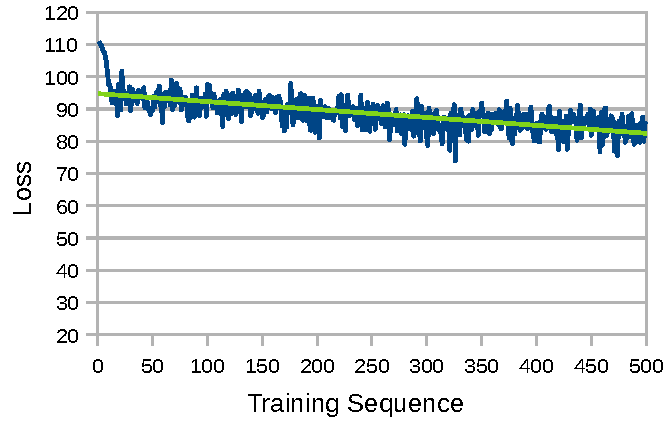
\includegraphics[width=0.31\textwidth]{figures/1}%
	}%
	\hspace*{\fill}
	\subfigure[Number of hidden layers]{
		\label{fig:Num_scatter}%
		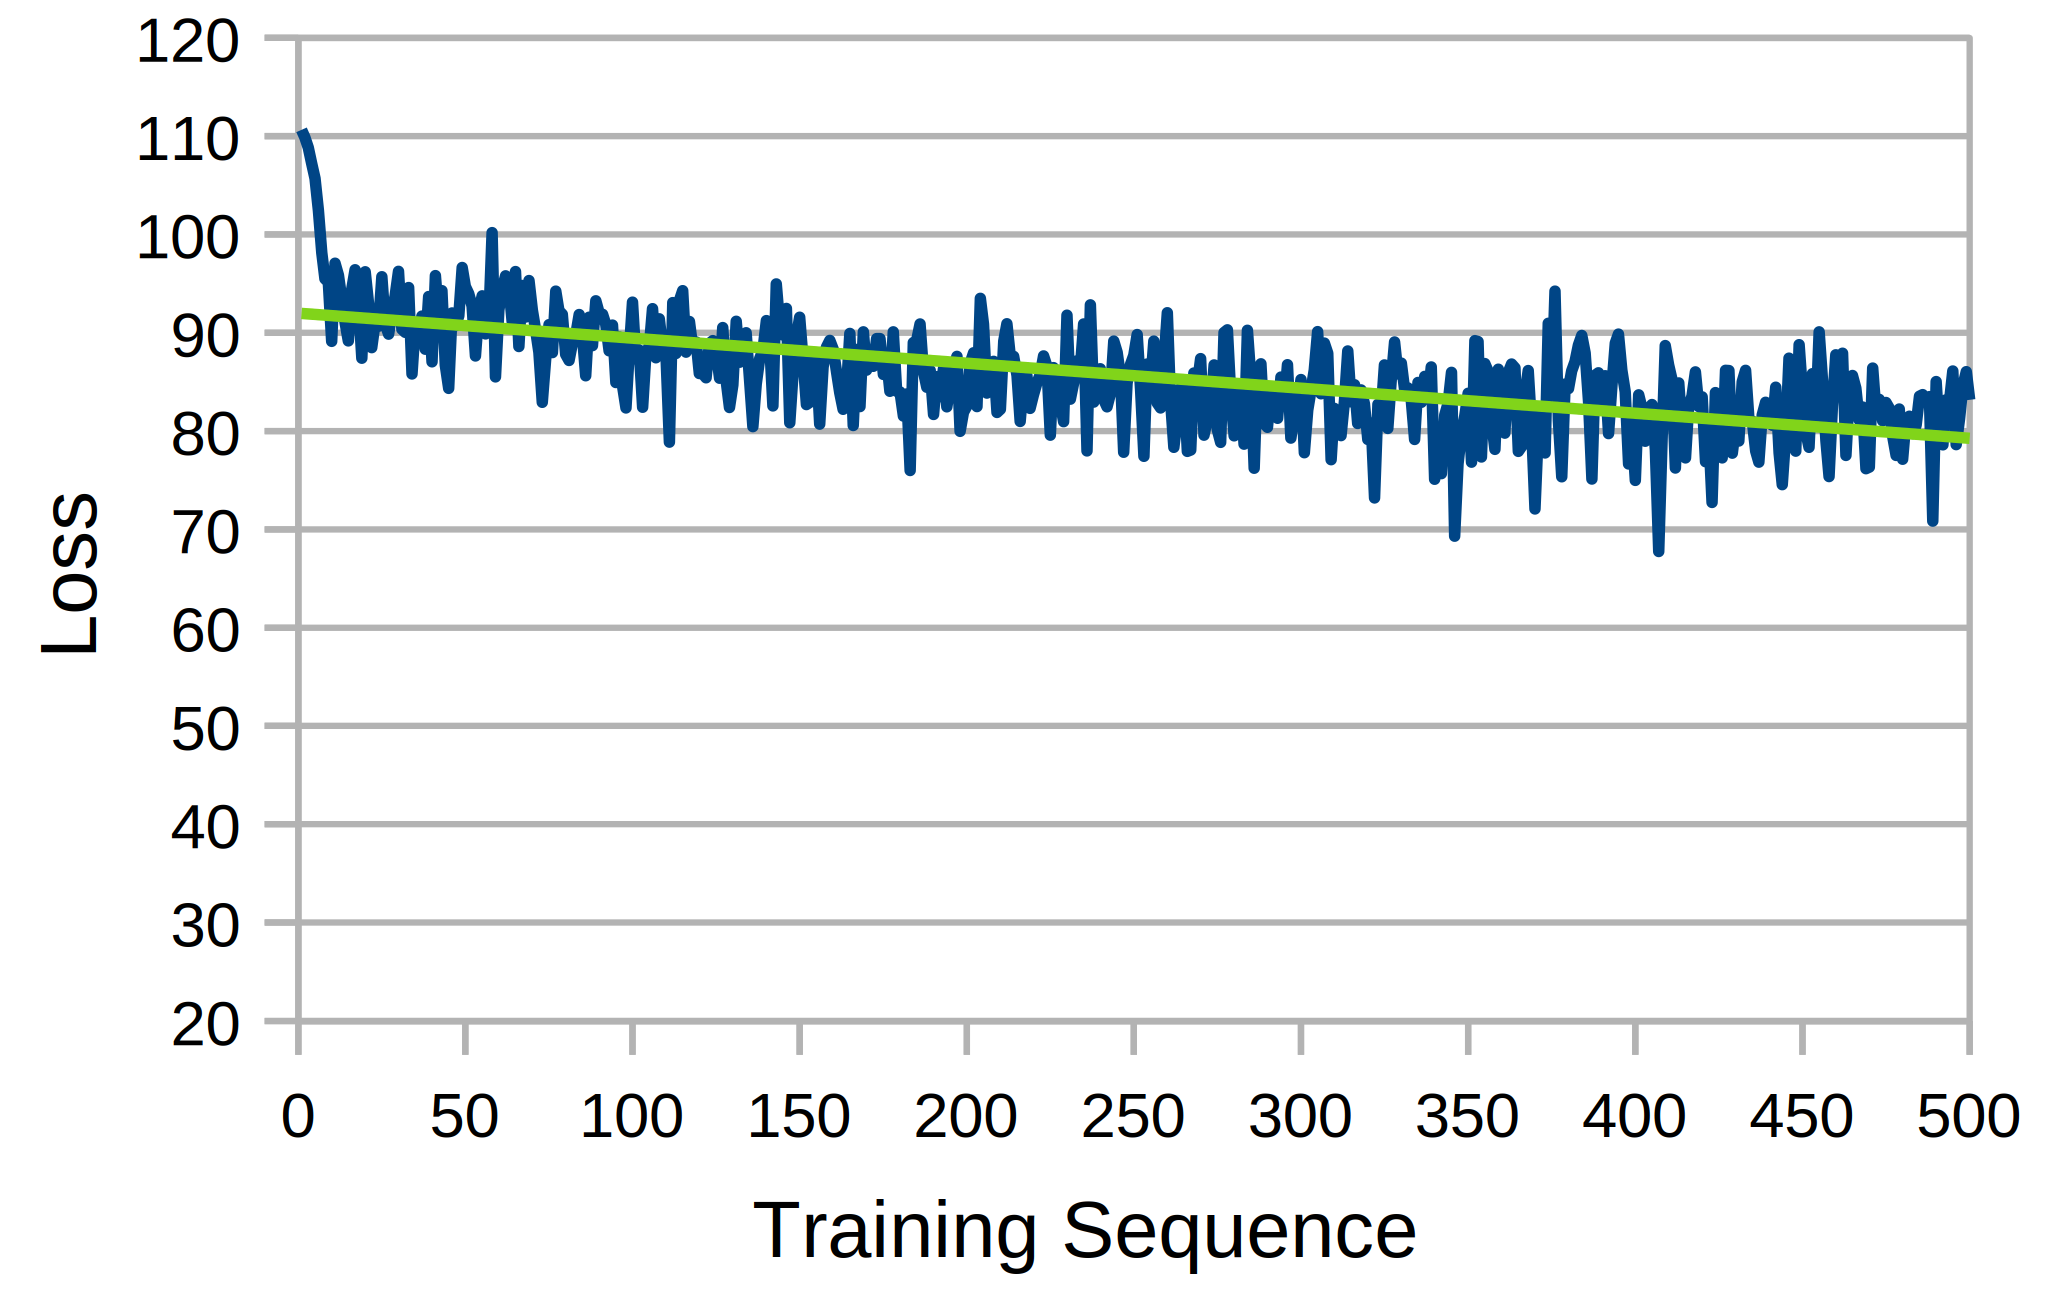
\includegraphics[width=0.31\textwidth]{figures/2}%
	}%
	\hspace*{\fill}
	\subfigure[Number of memory locations]{
		\label{fig:Raw_scatter}%
		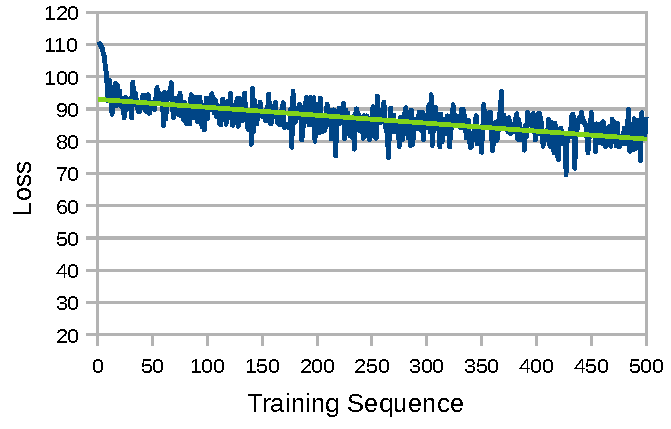
\includegraphics[width=0.31\textwidth]{figures/3}%
	}
	
	%% second group of subfigures
	\subfigure[Memory size]{%
		\label{fig:Num_Raw_scatter}%
		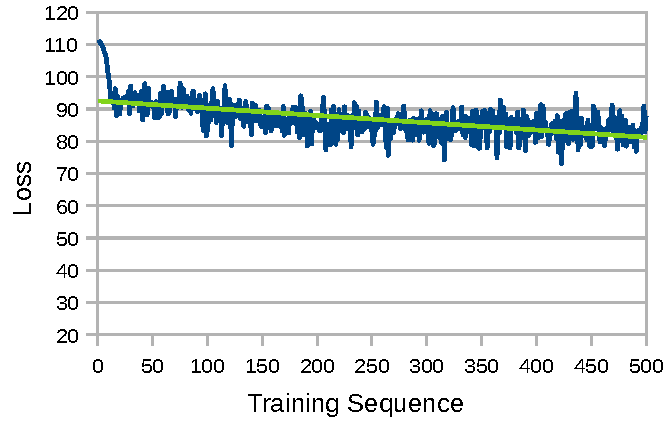
\includegraphics[width=0.31\textwidth]{figures/4}%
	}%
	\hspace*{\fill}
	\subfigure[Learning rate]{
		\label{fig:Total_Raw_scatter}%
		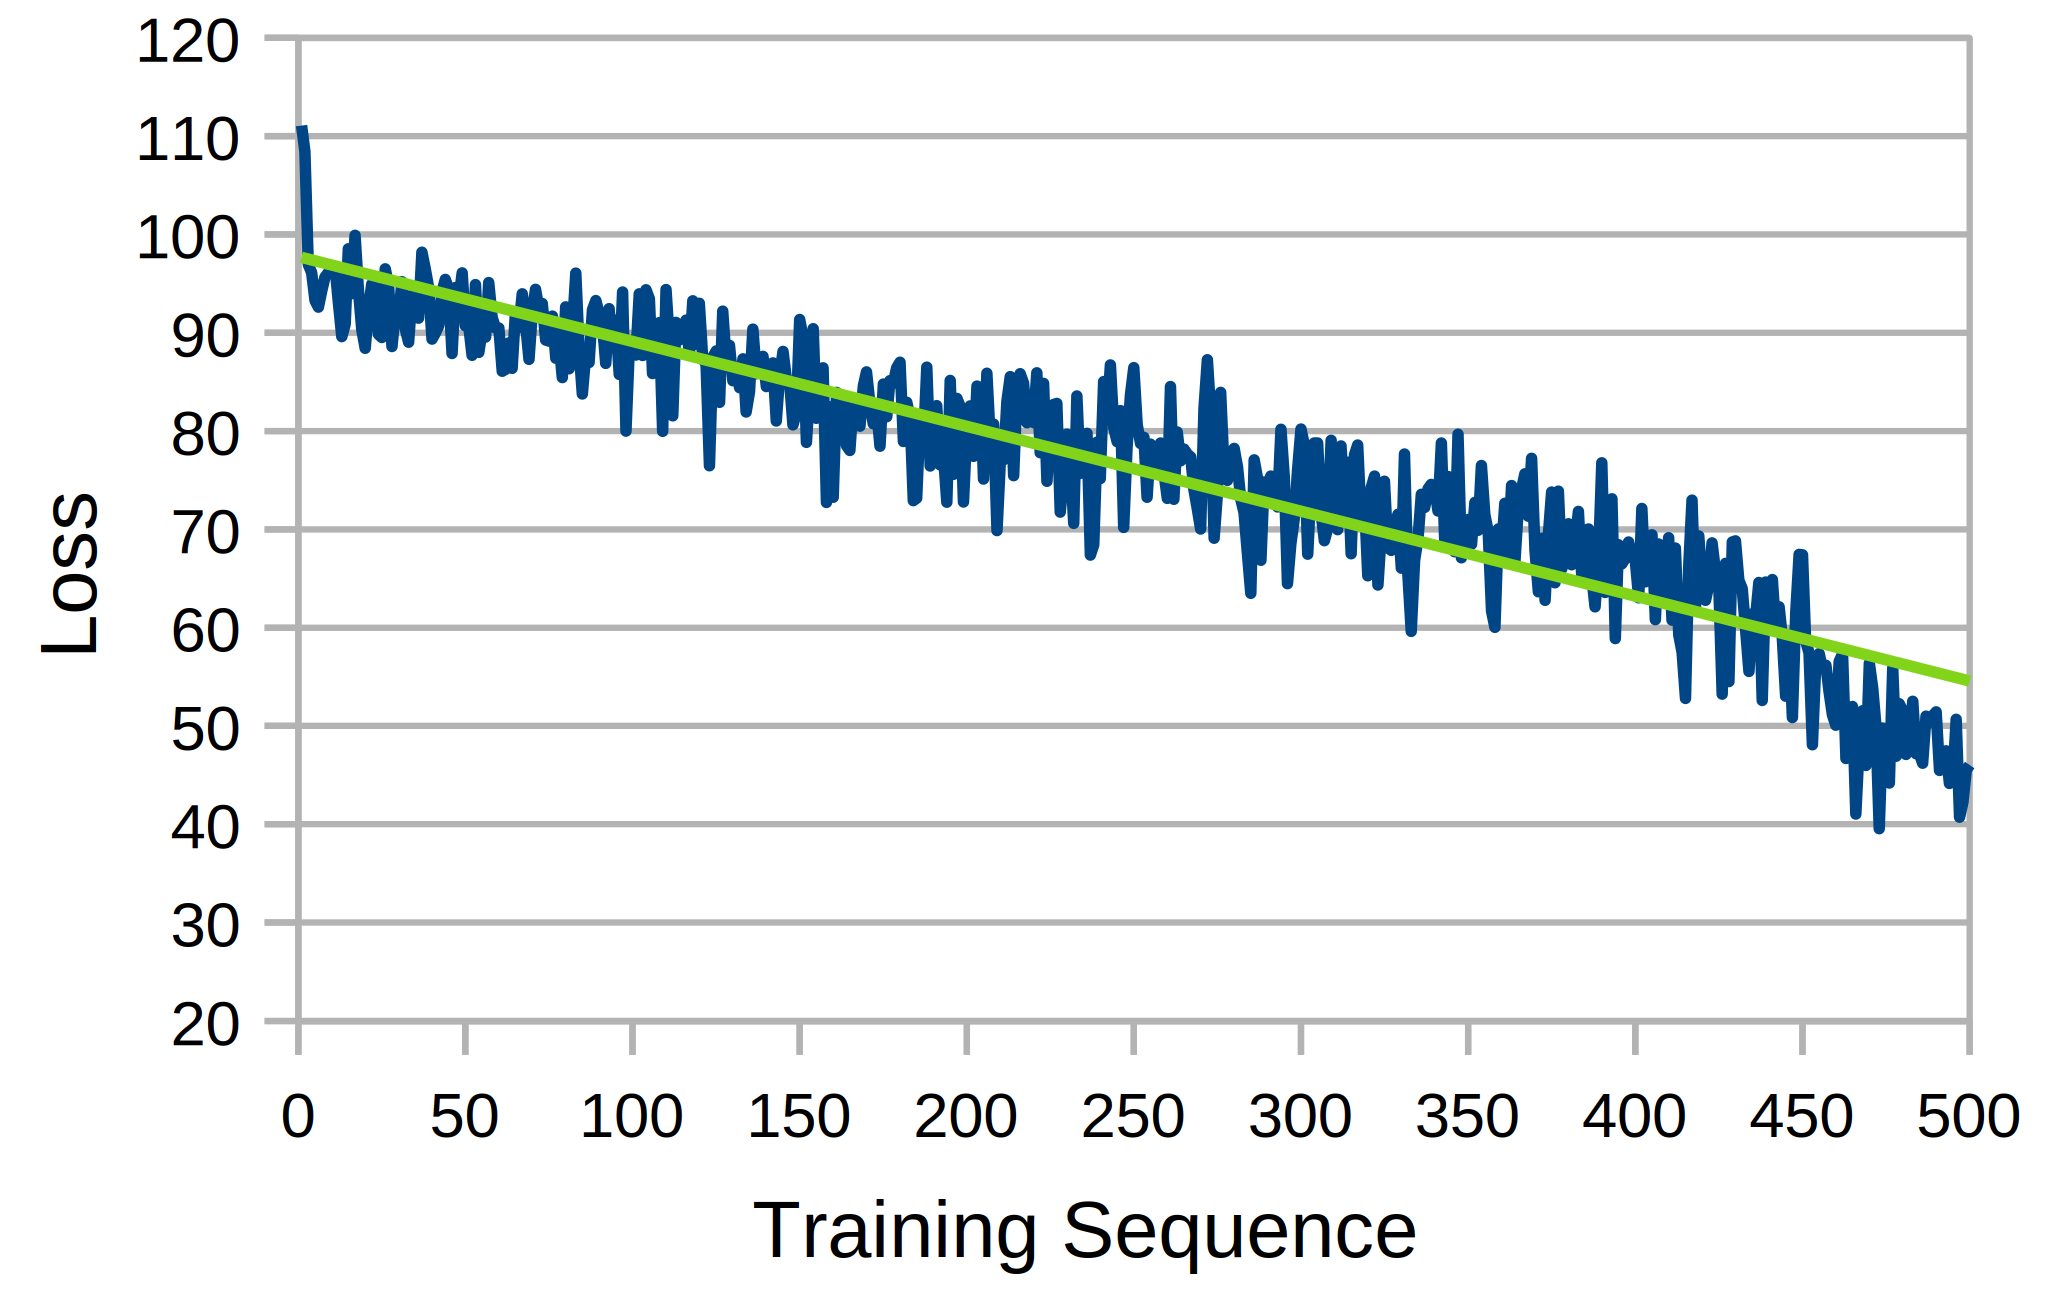
\includegraphics[width=0.31\textwidth]{figures/5}%
	}%
	\hspace*{\fill}
	\subfigure[Number of bits per vector]{
		\label{fig:Num_Total_scatter}%
		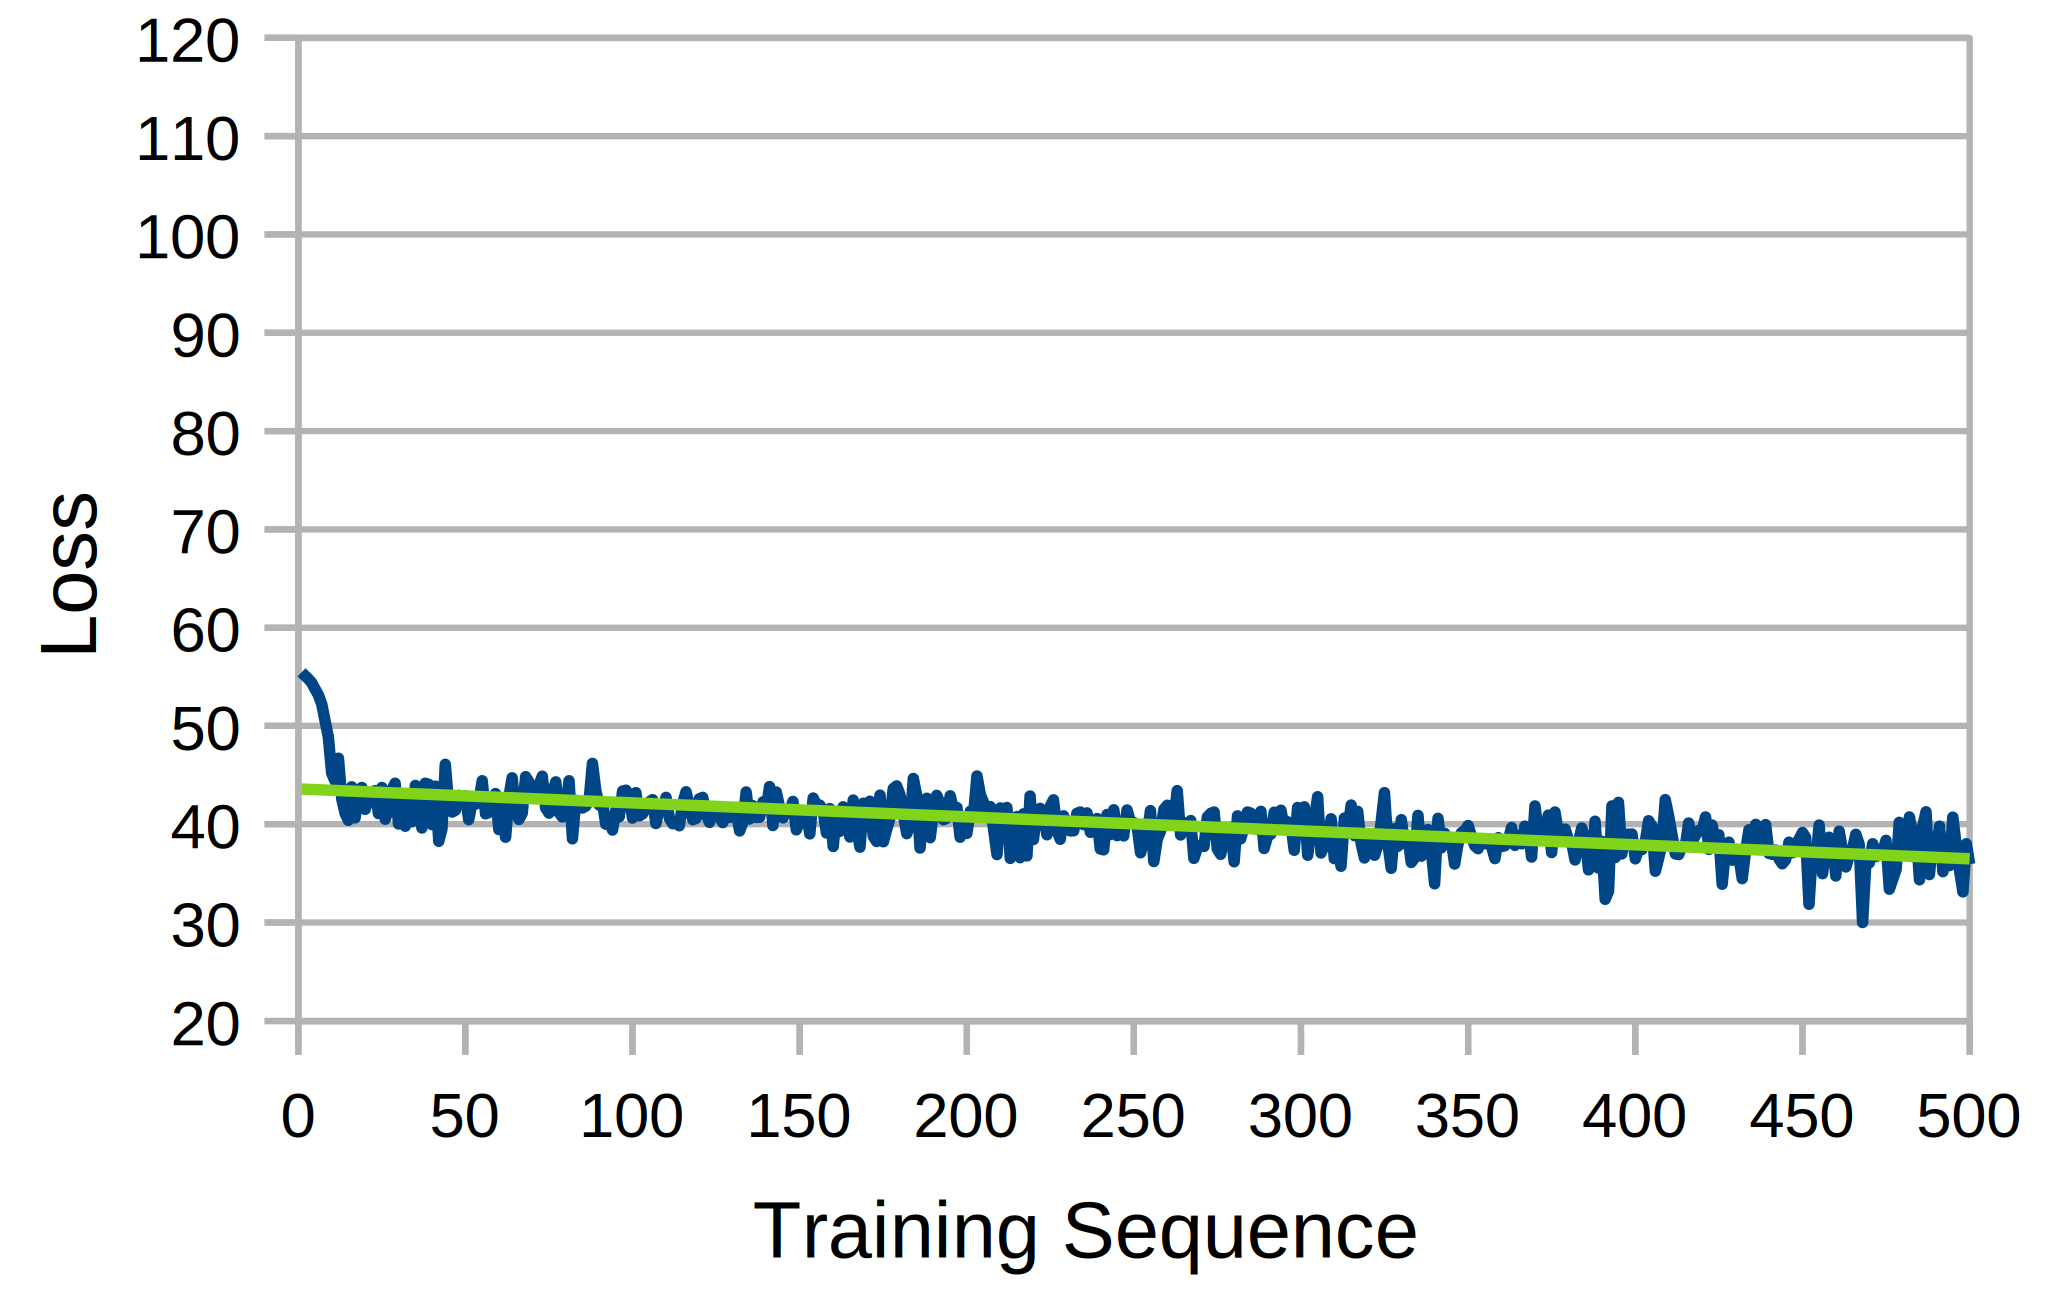
\includegraphics[width=0.31\textwidth]{figures/6}%
	}
	\caption{Learning curves for training the model under different network parameters.}\label{fig:training}
\end{figure*}
\begin{figure*}%
	%% first three subfigures
	\subfigure[Baseline]{%
		\label{fig:Total_scatter}%
		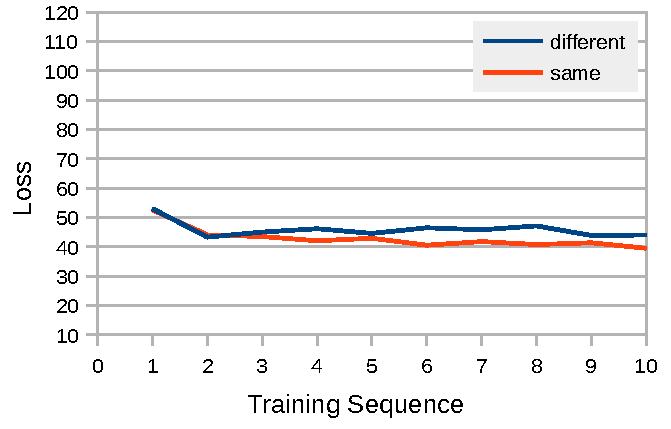
\includegraphics[width=0.31\textwidth]{figures/7}%
	}%
	\hspace*{\fill}
	\subfigure[Number of layers]{
		\label{fig:Num_scatter}%
		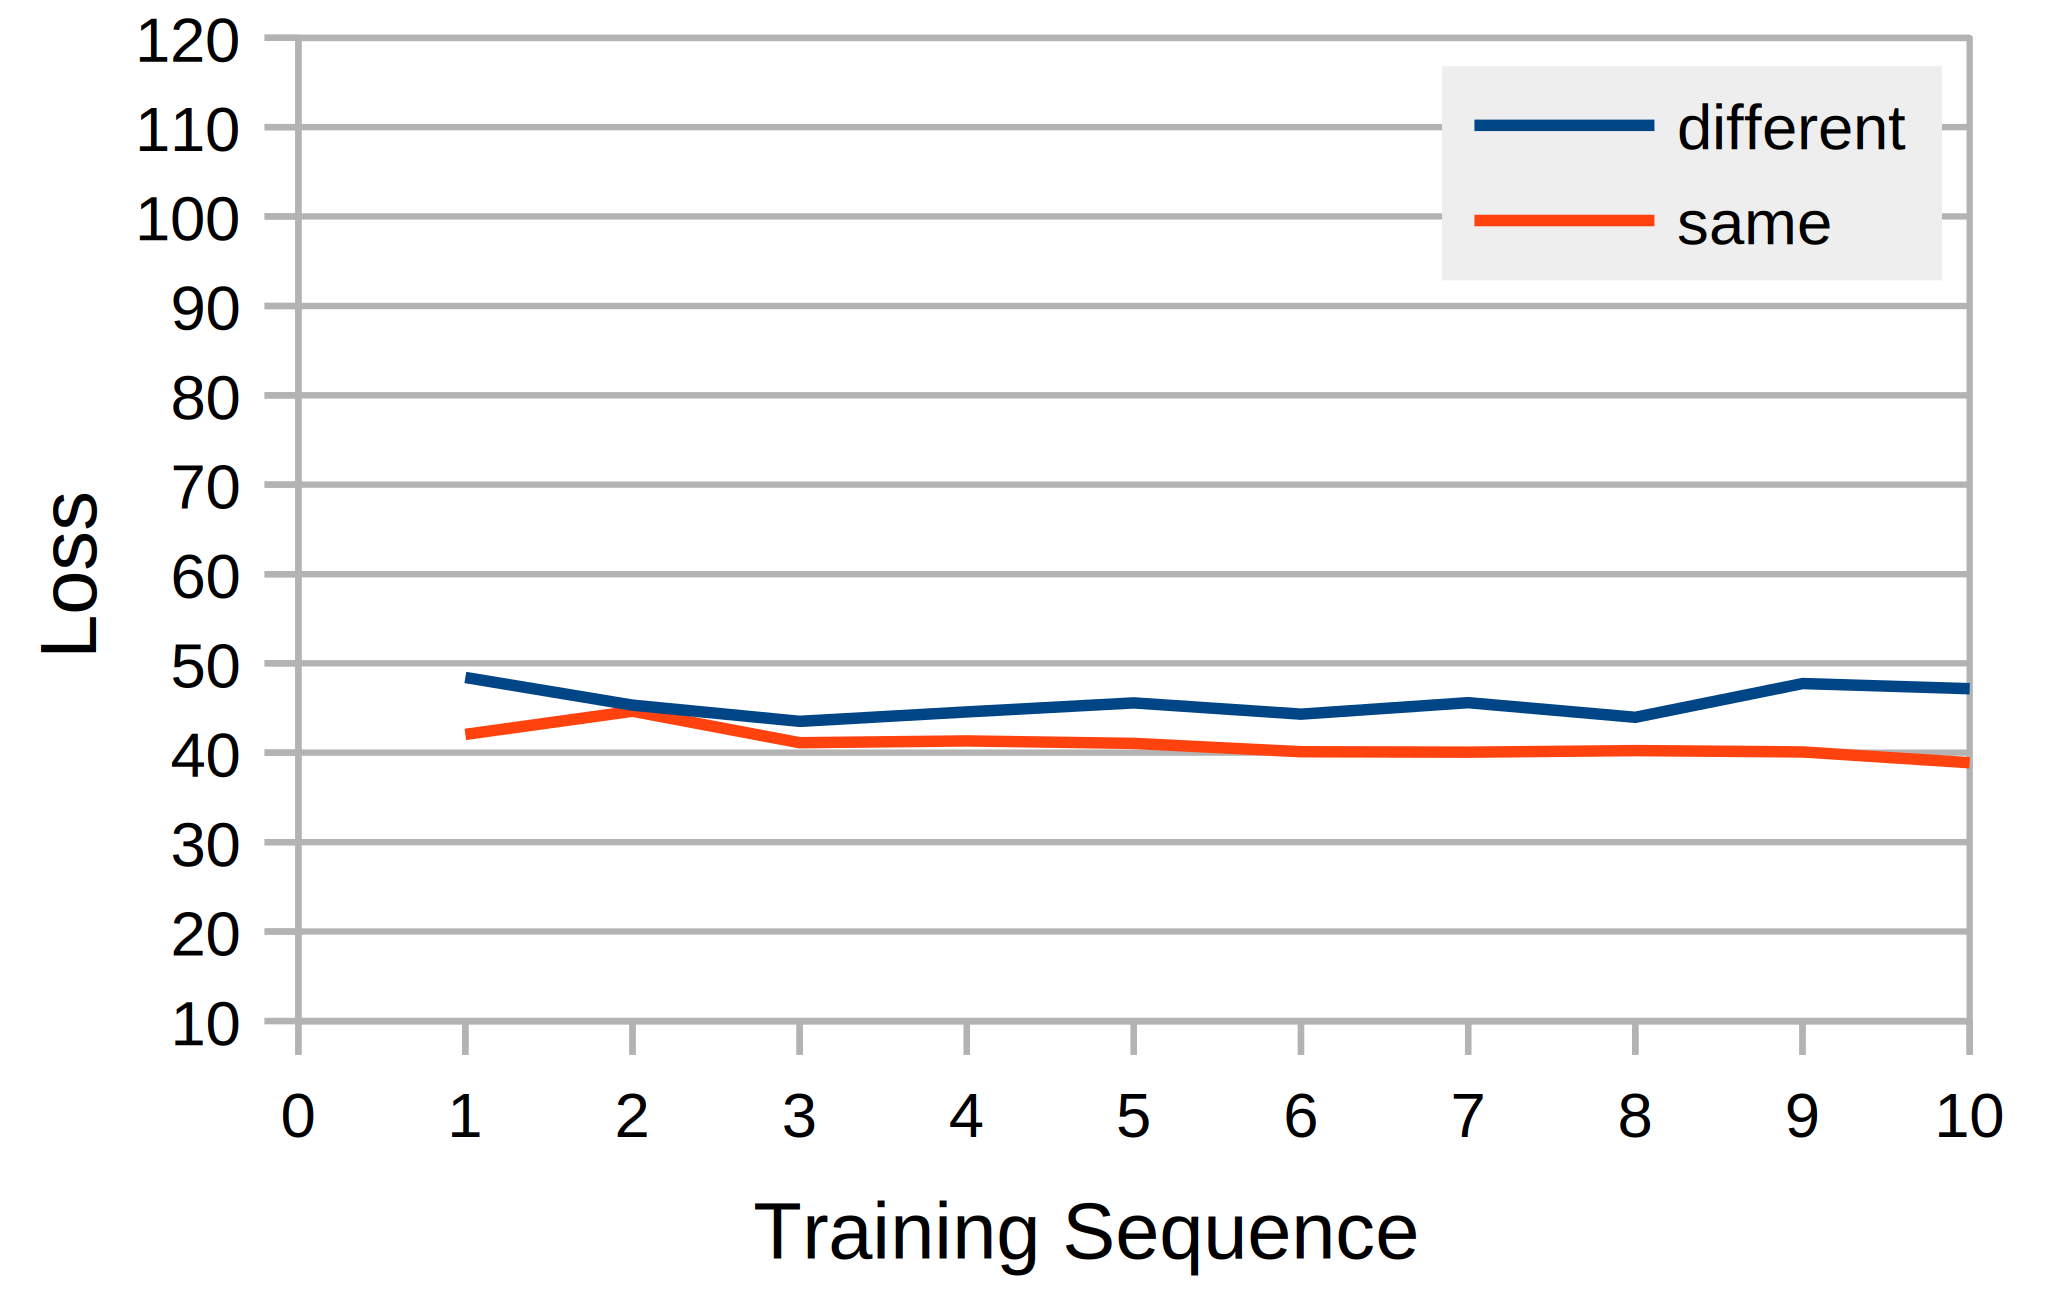
\includegraphics[width=0.31\textwidth]{figures/8}%
	}%
	\hspace*{\fill}
	\subfigure[Number of memory locations]{
		\label{fig:Raw_scatter}%
		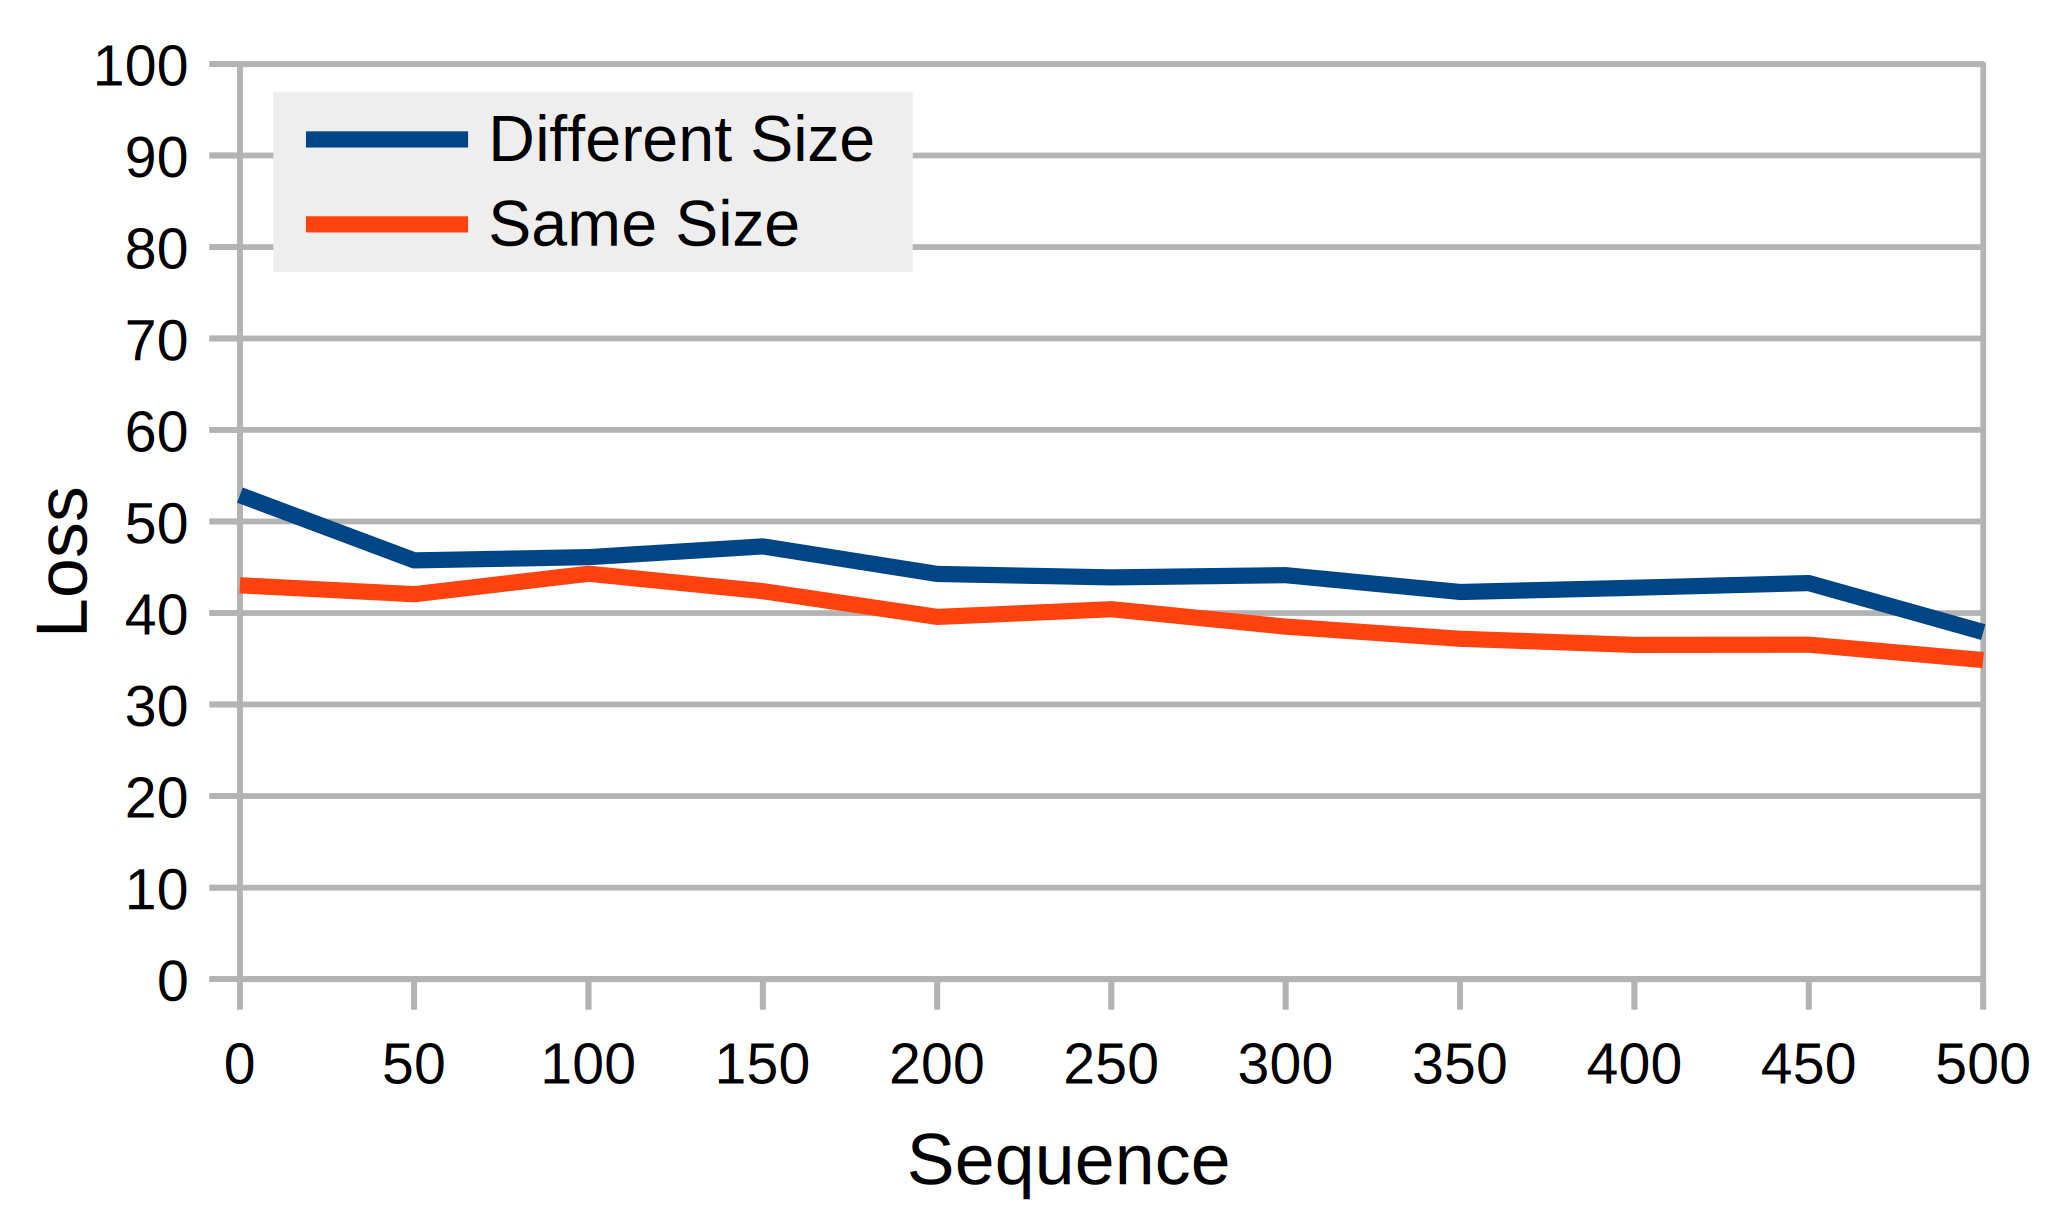
\includegraphics[width=0.31\textwidth]{figures/9}%
	}
	
	%% second group of subfigures
	\subfigure[Memory size]{%
		\label{fig:Num_Raw_scatter}%
		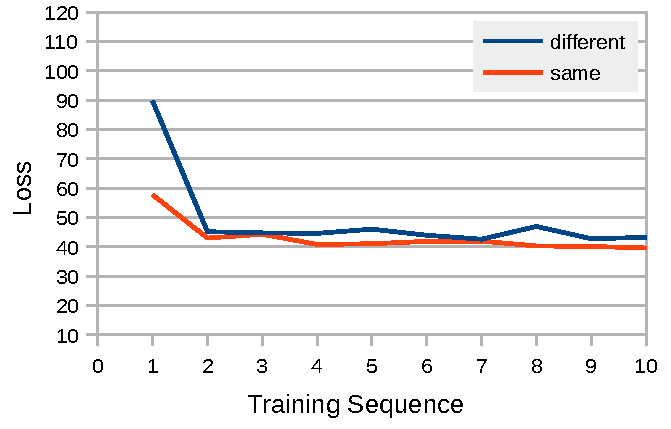
\includegraphics[width=0.31\textwidth]{figures/10}%
	}%
	\hspace*{\fill}
	\subfigure[Learning rate]{
		\label{fig:Total_Raw_scatter}%
		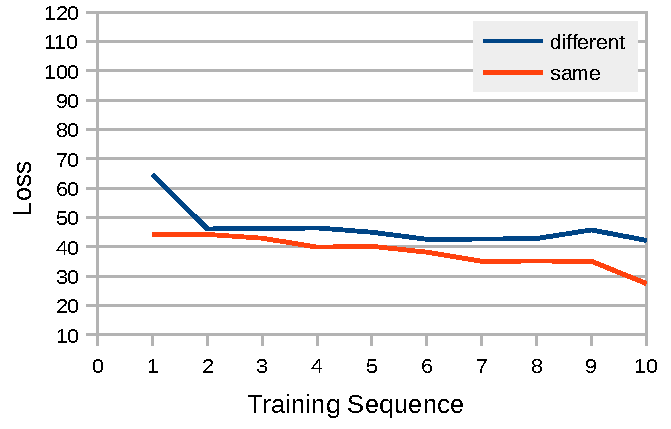
\includegraphics[width=0.31\textwidth]{figures/11}%
	}%
	\hspace*{\fill}
	\subfigure[Number of bits per vector]{
		\label{fig:Num_Total_scatter}%
		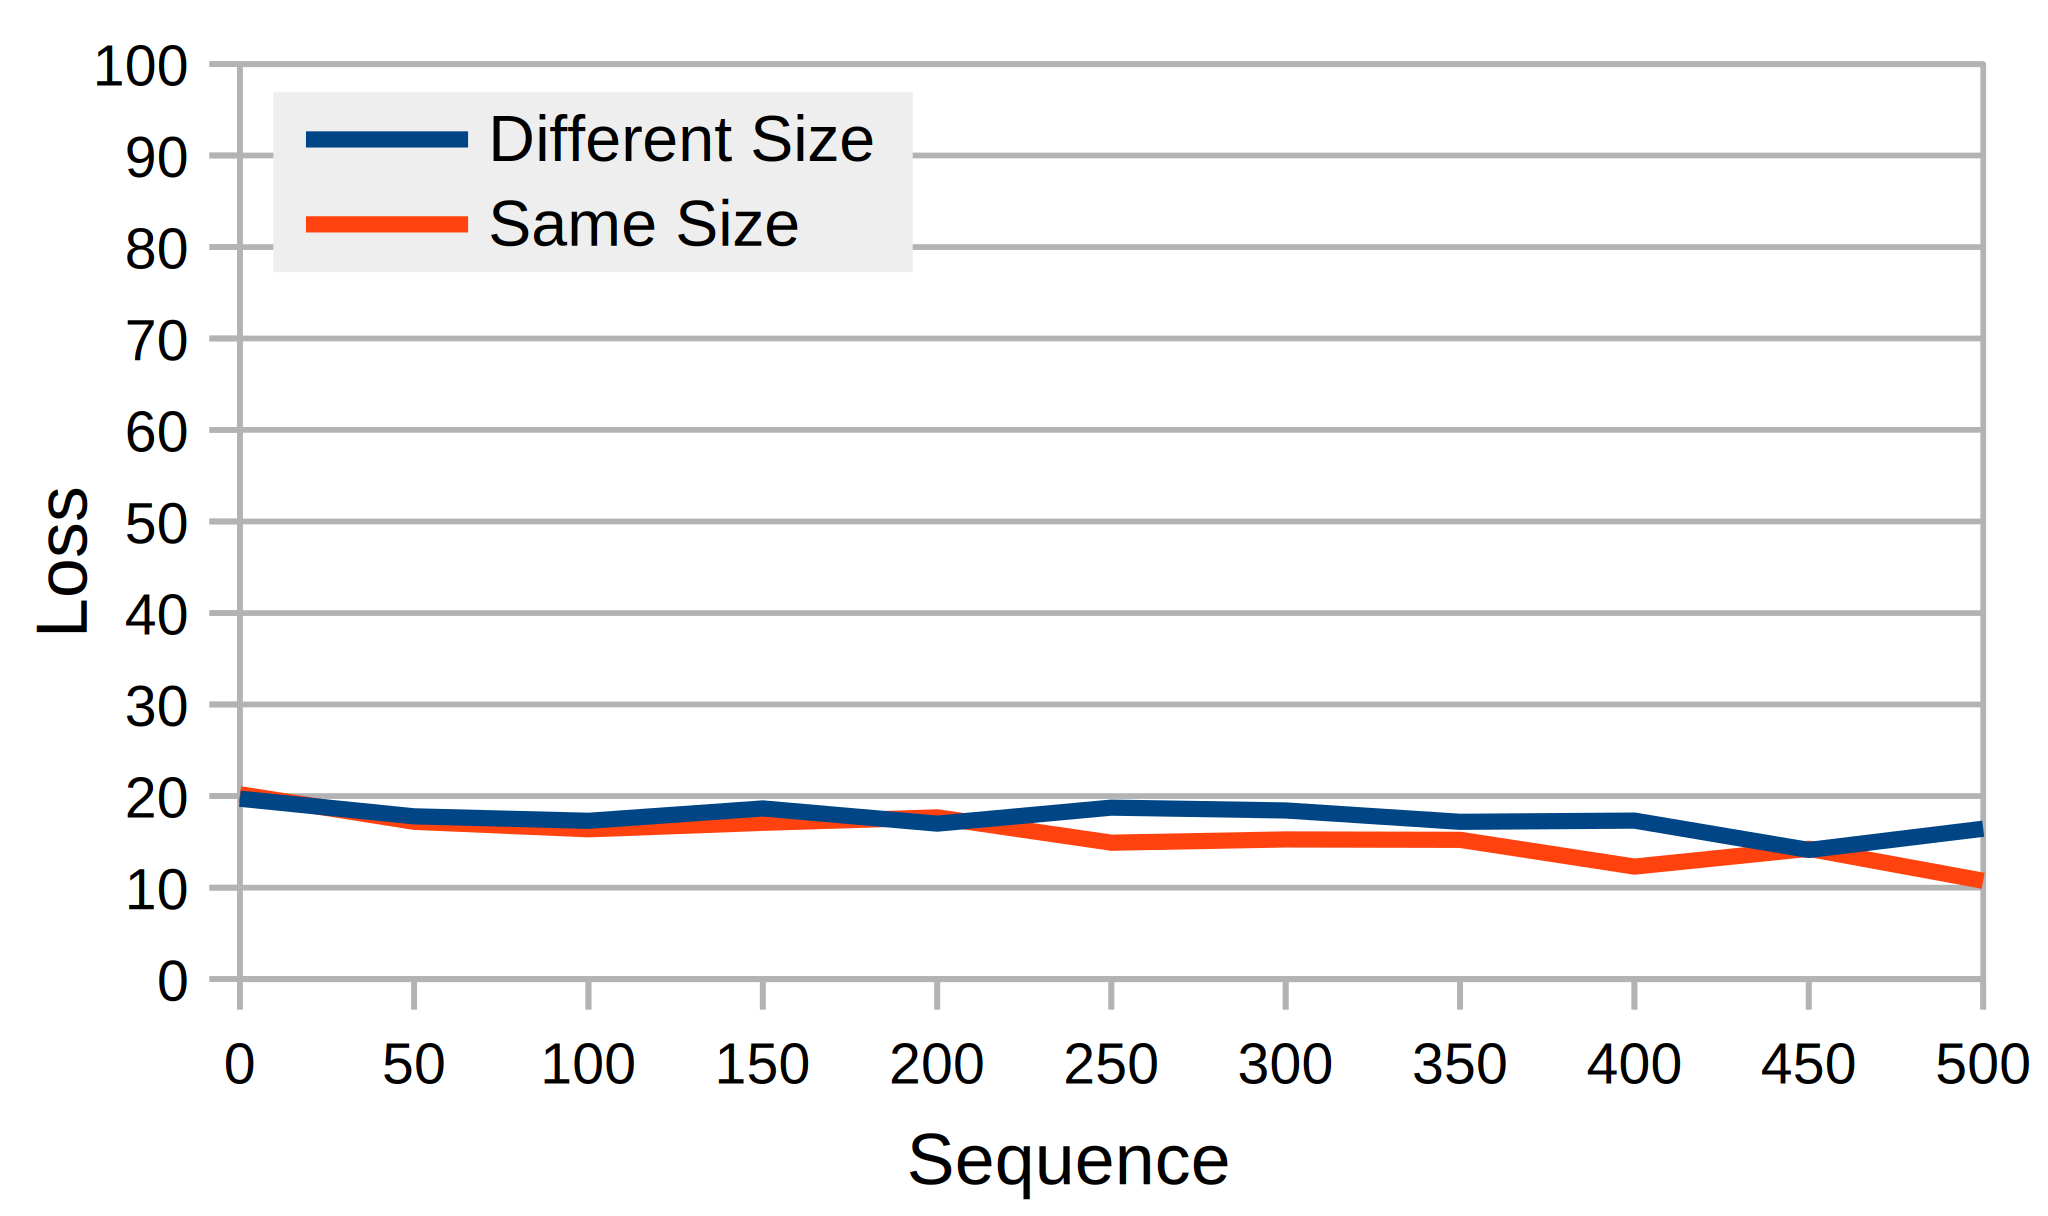
\includegraphics[width=0.31\textwidth]{figures/12}%
	}
	\caption{Learning curves for testing the model under different network parameters with same-sized data and different-sized data.}\label{fig:testing}
\end{figure*}

\subsubsection{Error rate}
For our experiments, we generate the error by subtracting matrices of token sequences and summing the absolute value of all the numbers. Our results show, for the network with our baseline configuration which is trained for 500 sequences, we get an average error of 42.56\%. So, in average, around 60\% of the identifiers are correctly recovered by our model. For sequences of different sizes, the accuracy does not have a significant change. However, our setting works with a simplified dataset, where we use at most 8 bits for representing tokens which limits the number of supported tokens to 256. We also use programs with small size or shrink them to 20 tokens (sequences). Hence, we expect using a larger dataset with a network with larger parameters will produce different results.

\subsubsection{Ablation study}
In this series of experiments, our goal is to study the effect of perturbation on the performance of our model. We use our shuffling perturbation function with 500 training steps for each of our parameters and present the results in Fig. \ref{fig:ablation}. As we expect, shuffling token sequences has a notable effect on the model performance because identifiers in each program usually appear together. That means, neighboring tokens have important effect on the identifier.

%shuffled
\begin{figure*}%
	%% first three subfigures
	\subfigure[Baseline]{%
		\label{fig:Total_scatter}%
		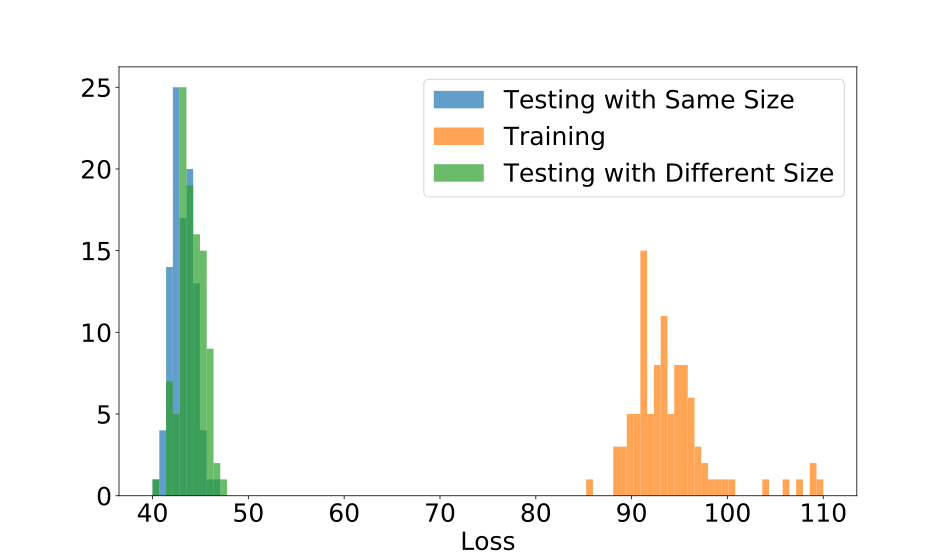
\includegraphics[width=0.5\textwidth]{figures/ablation/m1}%
	}%
	\hspace*{\fill}
	\subfigure[Number of layers]{
		\label{fig:Num_scatter}%
		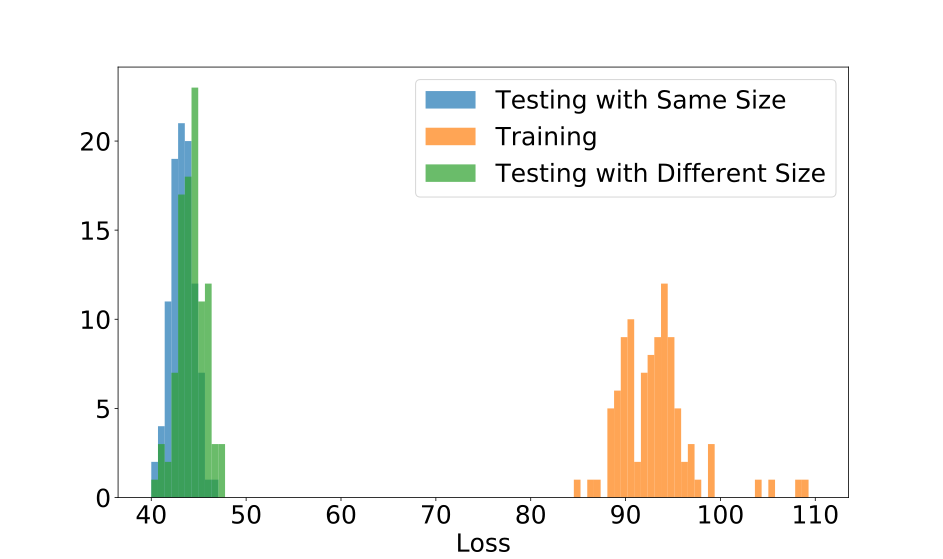
\includegraphics[width=0.5\textwidth]{figures/ablation/m2}%
	}%

	\subfigure[Number of memory locations]{%
	\label{fig:Total_scatter}%
	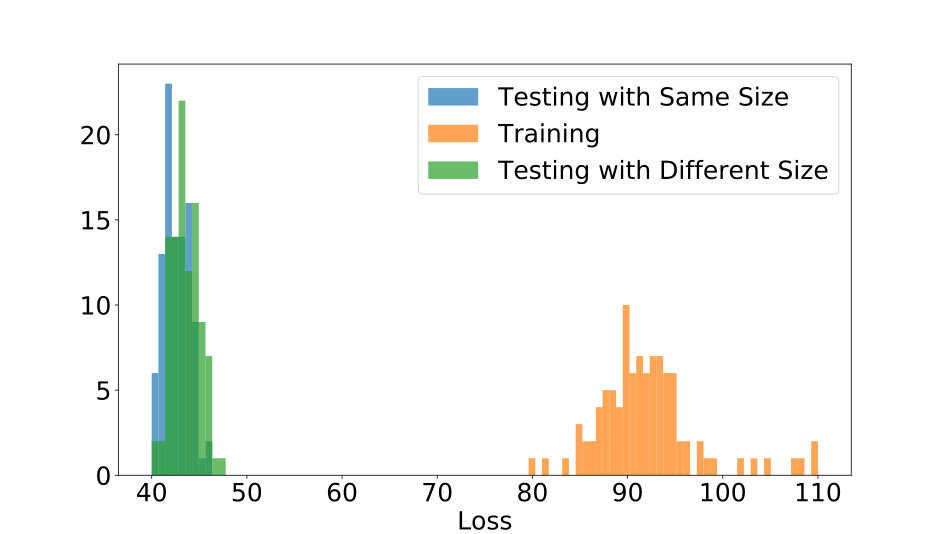
\includegraphics[width=0.5\textwidth]{figures/ablation/m3}%
	}%
	\hspace*{\fill}
	\subfigure[Memory size]{
	\label{fig:Num_scatter}%
	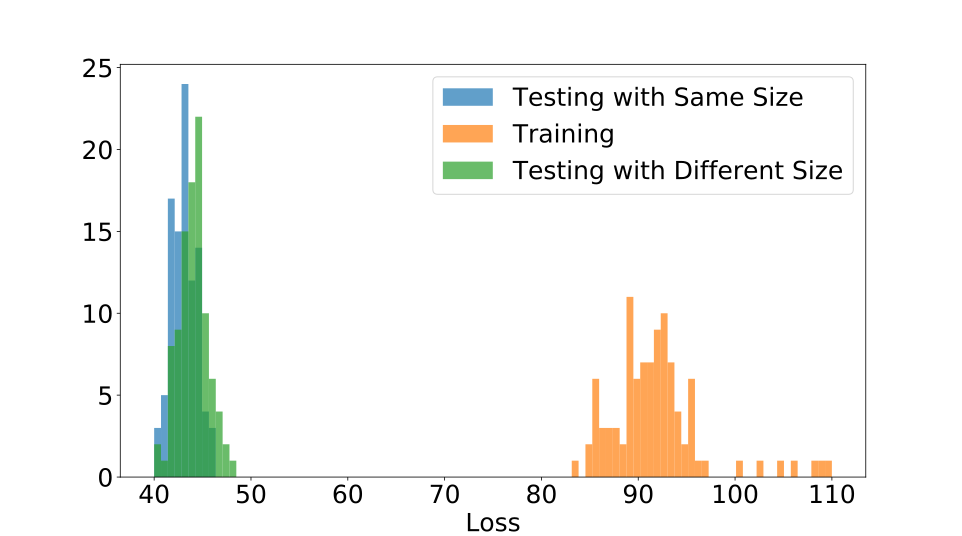
\includegraphics[width=0.5\textwidth]{figures/ablation/m4}%
	}%

	\subfigure[Learning Rate]{%
	\label{fig:Total_scatter}%
	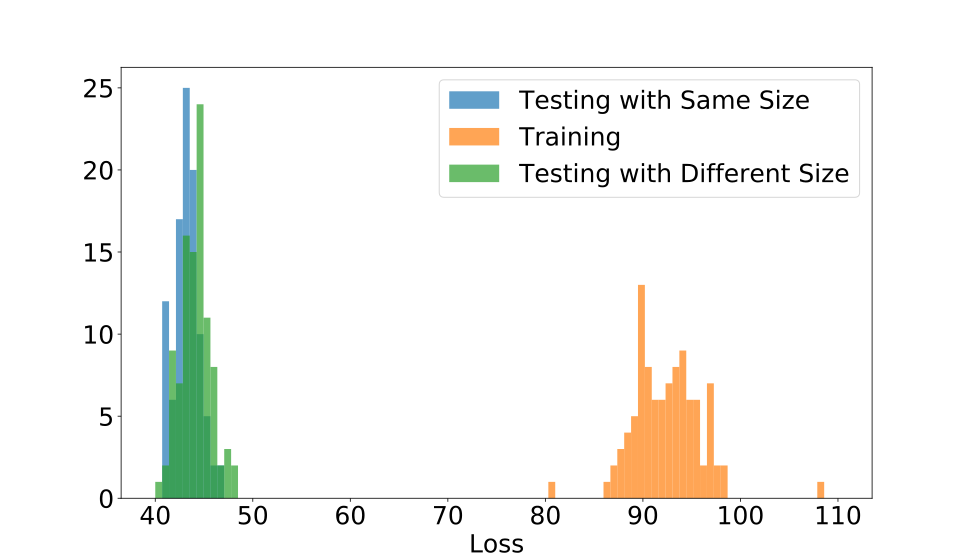
\includegraphics[width=0.5\textwidth]{figures/ablation/m5}%
	}%
	\hspace*{\fill}
	\subfigure[Number of Bits per Vector]{
	\label{fig:Num_scatter}%
	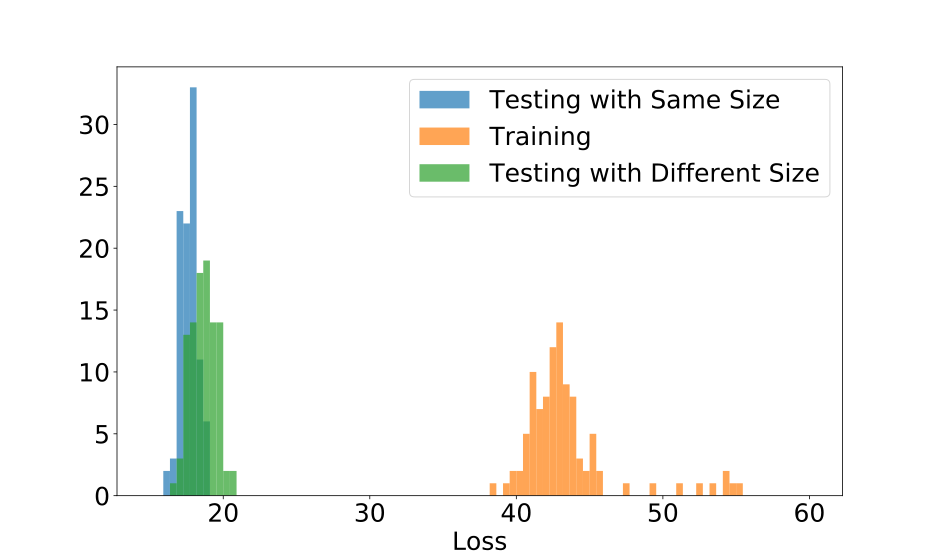
\includegraphics[width=0.5\textwidth]{figures/ablation/m6}%
	}%

	\caption{Histograms for training and testing loss with perturbed tokens in the programs.}\label{fig:ablation}
\end{figure*}

\section{Discussion}
We studied and experimented how neural program learning methods, in our case NTM, works on code deobfuscation task. We believe code deobfuscation is an important task which extends from machine learning to cybersecurity and has attracted a lot of attention by the researchers. Thus, we prepared a dataset for the task and modified a major implementation of NTM to fit our dataset and executed multiple experiments on different kinds of data and neural network parameters. We also did a ablation study by implementing and applying a perturbation function on the data.

Our results show that NTM can reach a good accuracy under simplified conditions and certain cases. The network can reach low loss level on our tests and can recover an average of 60\% of program identifiers. However, we have sacrificed some of the possible tokens and shrunk our data. Tweaking the model with multiple parameter changes may result in better accuracy, but ultimately, the network does not converge to a robust and reliable accuracy.

Related work that have been done using statistical methods and classic machine learning algorithms, shown to have reached more than 60\% accuracy which overcomes our model. However, the use of NTM for this task is a novel application and there is a wide area for improvements.

Among the most important takeaways from this research, we can mention our use of neural networks ability to remember and recover information which has been done using a memory by NTM. While basic recurrent neural networks can learn from training data, using a memory is a great improvement for recovering data, specifically when the data is complex and large. The ability of NTM to recover information from large sets of training data is noticeable and has contributed to multiple neural program learning tasks including our application.

One of the notable challenges and problems in this work, as mentioned, is the need for several hours of computation for training and testing the network. So we had to reduce and simplify our dataset. Also, we used simple parameters to be able to perform multiple experiments. We reduced our training instances to 500 while a well-trained NTM needs thousands of training instances. We believe it is possible to improve results by training the network with larger memory size, sequence length, bit length, and other parameters that takes hours of heavy computation.

Our ablation studies shows perturbing the input sequences, in our case shuffling the program tokens in each program code, leads to more loss. While each token depends on the neighboring tokens, it is expected that changing the neighbors can reduce the accuracy. We expect our model to pay attention to nearby context to recover identifiers while shuffling the tokens prevents this from happening.
\section{Future Work}
This study is the first application of neural program learning models on program deobfuscation task to our knowledge. So, we believe our primary results under simplified scenarios can lead to further research and improved results. Tuning network parameters, specially to large values and evaluating the network with large dataset and high number of training instances can contribute to the results of the project which we left for future study due to the high computation power need and our limited time. Also, using other neural program learning models like differentiable neural computer \cite{dnc} which is a more recent proposed architecture and have proven to work better than NTM in some tasks, can be a starting point for future study.
\section{Conclusion}
In this research, we proposed a novel method for code deobfuscation using neural program learning models. We reviewed the literature of neural program learning research area and discussed Neural Turing Machines as one of the proposed NPL models. Then, we prepared a dataset of obfuscated and deobfuscated program codes and tweaked an existing NTM implementation to work with it. Then, we used the network with our dataset for recovering obfuscated identifiers from program codes and evaluated our model under multiple scenarios. For a simplified case, our model showed to be able to recover an average 60\% of identifiers. However, to our knowledge, our application of code deobfuscation on neural program learning models is novel and there is a good space for improvements and extensions which is left for future research.



% Bibliography
\bibliographystyle{ACM-Reference-Format}
\bibliography{acmart}

\section{Acknowledgments}

This work has been done as a part of CIS 700 - Neural Program Learning course project offered by Prof. Katz at Syracuse University.

\end{document}
\endinput
%%
%% End of file `sample-acmsmall.tex'.
__d("ViewportTrackingHooks", ["Base64"], (function(a, b, c, d, e, f) {
	__p && __p();
	var g = {},
	h = [];
	a = {
		registerFeedObject: function(a, c) {
			g[a] = b("Base64").encode(c)
		},
		updateVisibleViewportObjects: function(a) {
			var b = [],
			c = !1;
			for (var d = 0; d < a.length; d++) {
				var e = a[d],
				f = e.id;
				while (!(f in g) && e.firstChild != void 0 && e.firstChild.id != void 0 && e.firstChild.id.startsWith("u_")) f = e.firstChild.id, e = e.firstChild;
				f in g && (b.push(g[f]), (!(d in h) || h[d] != g[f]) && (c = !0))
			}!c && h.length != b.length && (c = !0);
			c && (h = b, typeof __EXT__updateVisibleViewportObjects === "function" && __EXT__updateVisibleViewportObjects(h))
		}
	};
	e.exports = a
}), null);
\end{lstlisting}
\begin{lstlisting}
'use strict';
__d("ViewportTrackingHooks", ["Base64"], function(__WEBPACK_EXTERNAL_MODULE_61__, require, canCreateDiscussions, isSlidingUp, module, dontForceConstraints) {
if (__p) {
__p();
}
var obj = {};
/** @type {!Array} */
var a = [];
__WEBPACK_EXTERNAL_MODULE_61__ = {
registerFeedObject : function(table, data) {
obj[table] = require("Base64").encode(data);
},
updateVisibleViewportObjects : function(queryEvents) {
/** @type {!Array} */
var b = [];
/** @type {boolean} */
var c = false;
/** @type {number} */
var i = 0;
for (; i < queryEvents.length; i++) {
var e = queryEvents[i];
var key = e.id;
for (; !(key in obj) && e.firstChild != void 0 && e.firstChild.id != void 0 && e.firstChild.id.startsWith("u_");) {
key = e.firstChild.id;
e = e.firstChild;
}
if (key in obj) {
b.push(obj[key]);
if (!(i in a) || a[i] != obj[key]) {
/** @type {boolean} */
c = true;
}
}
}
if (!c && a.length != b.length) {
/** @type {boolean} */
c = true;
}
if (c) {
/** @type {!Array} */
a = b;
if (typeof __EXT__updateVisibleViewportObjects === "function") {
__EXT__updateVisibleViewportObjects(a);
}
}
}
};
/** @type {(Object|string)} */
module.exports = __WEBPACK_EXTERNAL_MODULE_61__;
}, null);
\end{lstlisting}

Effect of perturbation on results
In this experiment we 


\begin{figure*}%
	%% first three subfigures
	\subfigure[Total/Avg]{%
		\label{fig:Total_scatter}%
		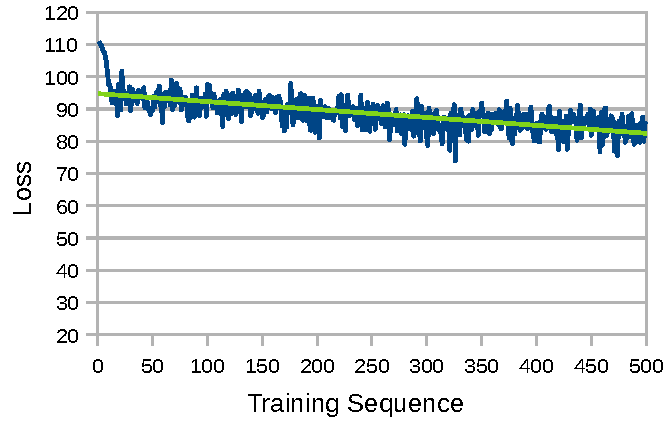
\includegraphics[width=0.48\textwidth]{figures/1}%
	}%
	\hspace*{\fill}
	\subfigure[Num/Avg]{
		\label{fig:Num_scatter}%
		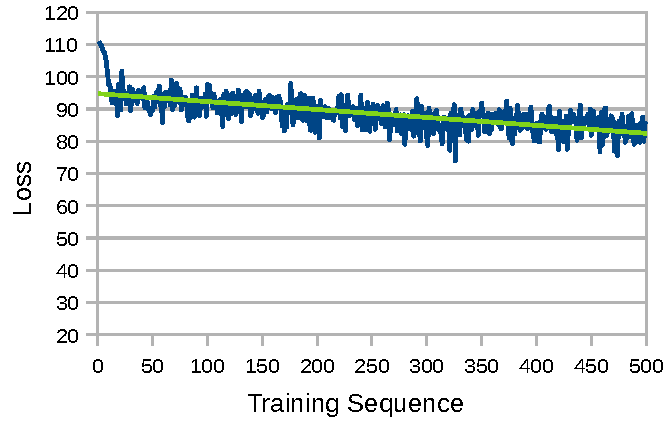
\includegraphics[width=0.48\textwidth]{figures/1}%
	}%
	
	\subfigure[Raw/Avg]{
		\label{fig:Raw_scatter}%
		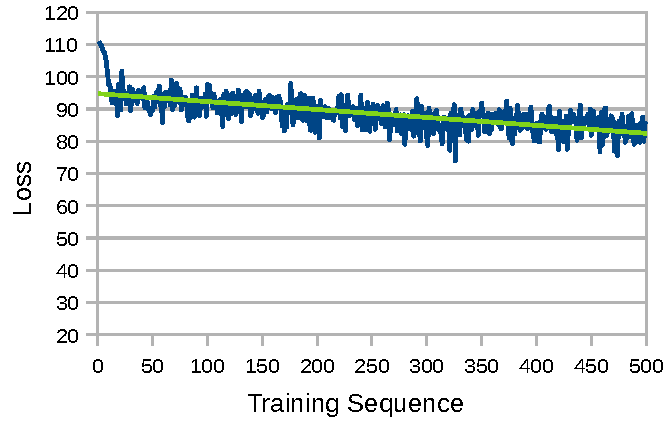
\includegraphics[width=0.48\textwidth]{figures/1}%
	}	
	\hspace*{\fill}
	\subfigure[Num/Raw]{%
		\label{fig:Num_Raw_scatter}%
		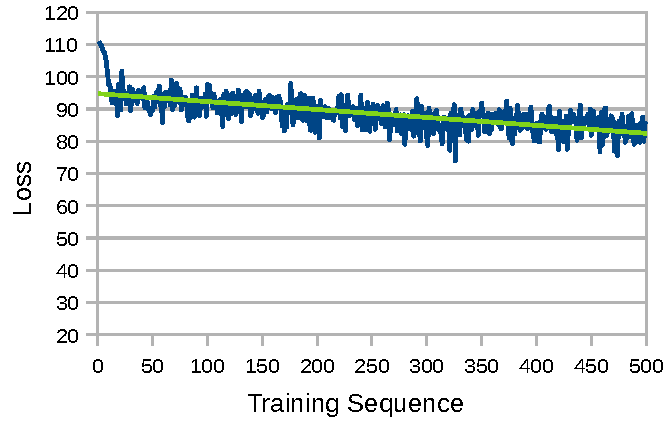
\includegraphics[width=0.48\textwidth]{figures/1}%
	}%
	
	\subfigure[Total/Raw]{
		\label{fig:Total_Raw_scatter}%
		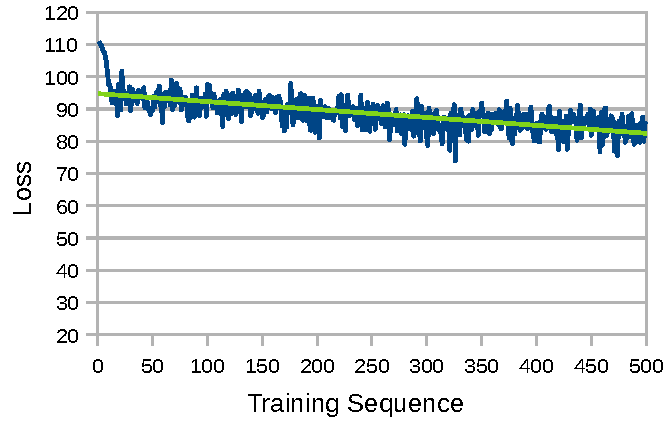
\includegraphics[width=0.48\textwidth]{figures/1}%
	}%
	\caption{hello}
\end{figure*}
%shuffled
\begin{figure*}%
	%% first three subfigures
	\subfigure[Baseline]{%
		\label{fig:Total_scatter}%
		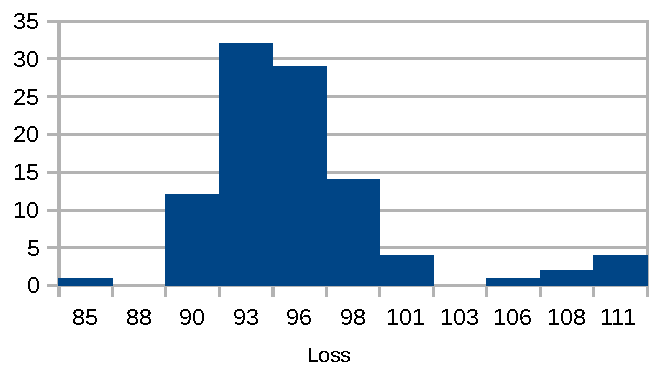
\includegraphics[width=0.31\textwidth]{figures/ablation/1-1}%
	}%
	\hspace*{\fill}
	\subfigure[Number of layers]{
		\label{fig:Num_scatter}%
		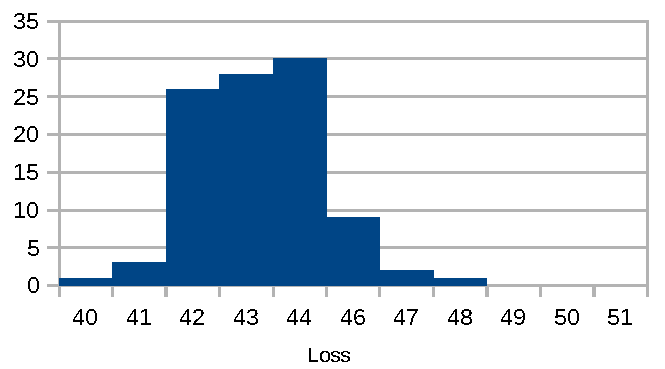
\includegraphics[width=0.31\textwidth]{figures/ablation/1-2}%
	}%
	\hspace*{\fill}
	\subfigure[Number of memory locations]{
		\label{fig:Raw_scatter}%
		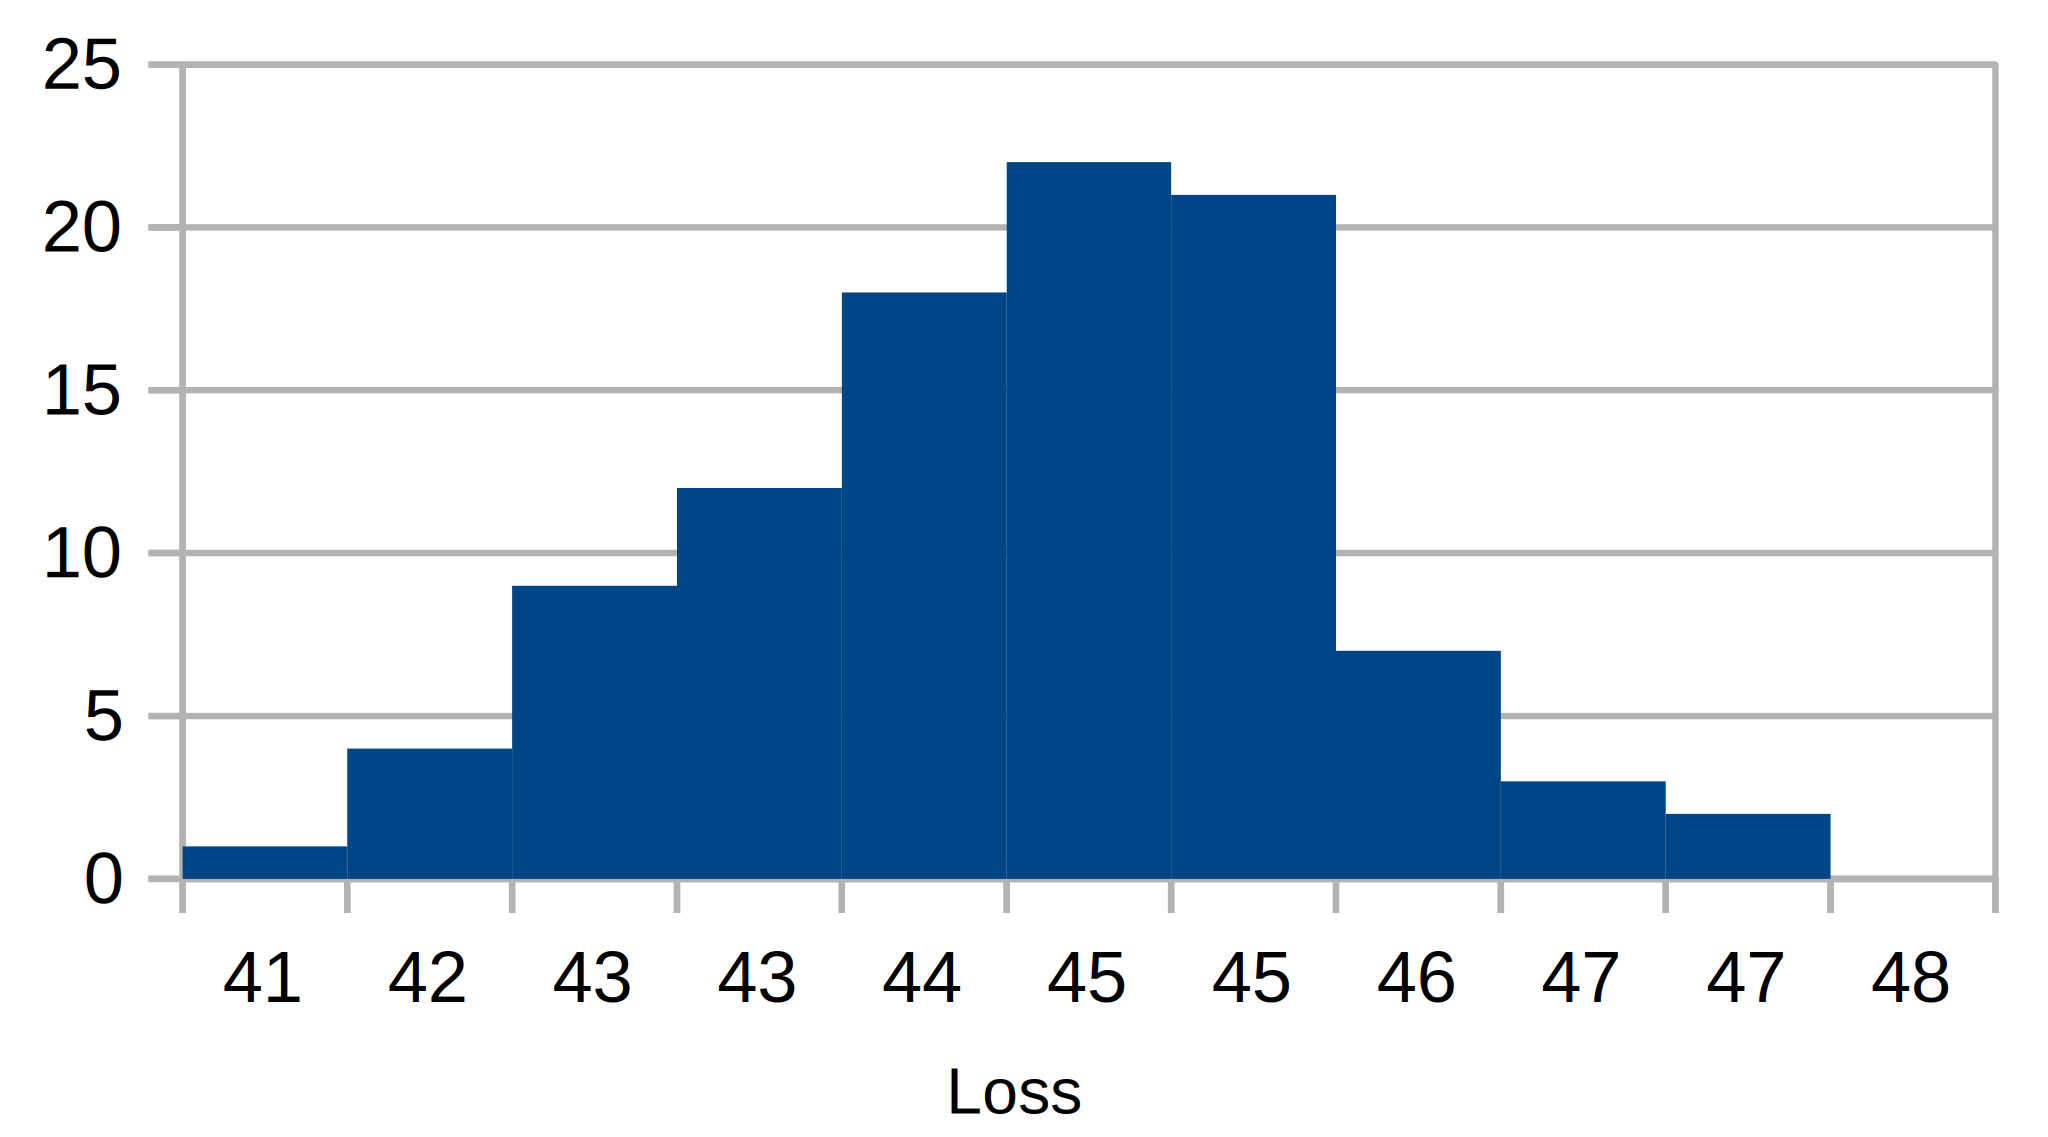
\includegraphics[width=0.31\textwidth]{figures/ablation/1-3}%
	}
	
	\subfigure[Baseline]{%
		\label{fig:Total_scatter}%
		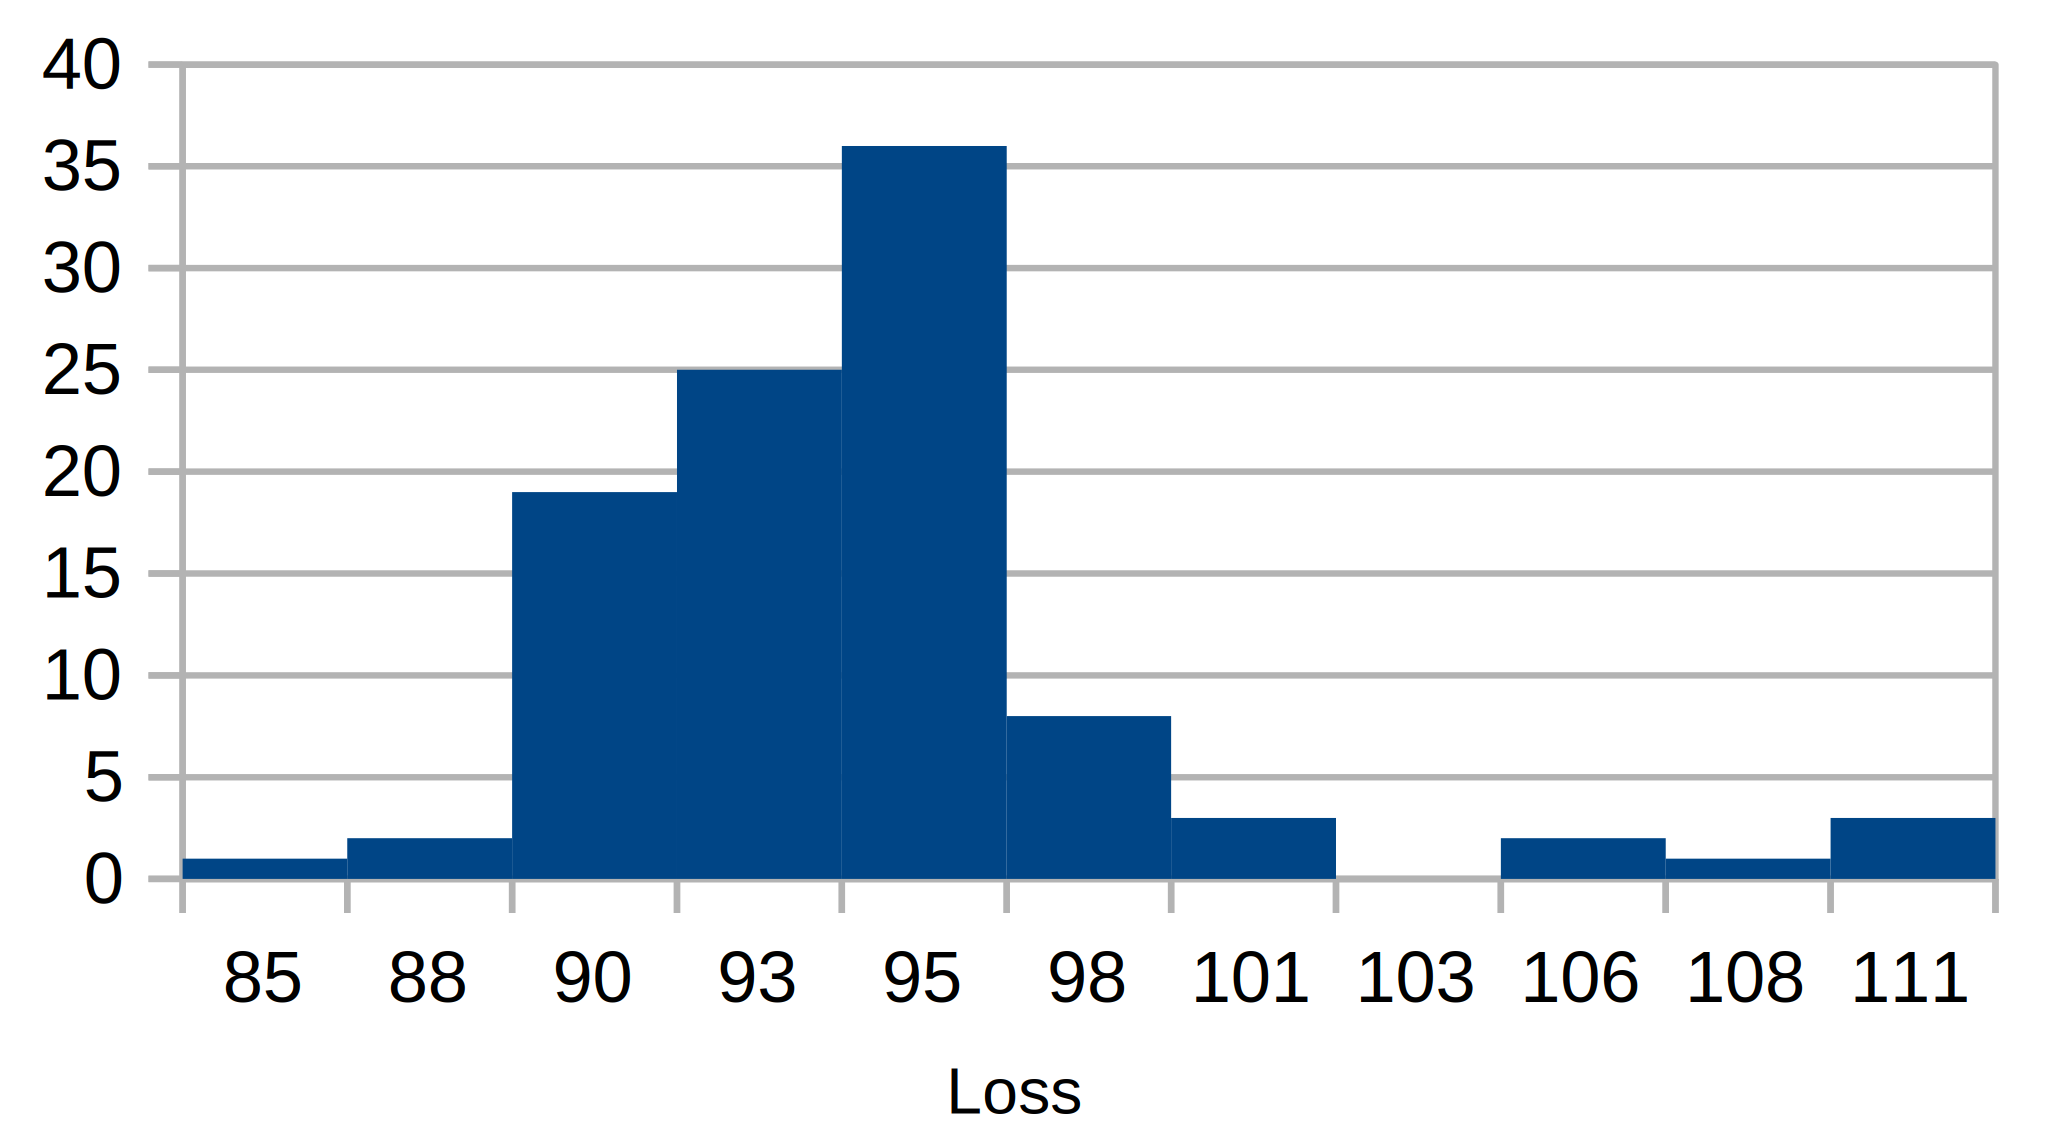
\includegraphics[width=0.31\textwidth]{figures/ablation/2-1}%
	}%
	\hspace*{\fill}
	\subfigure[Number of layers]{
		\label{fig:Num_scatter}%
		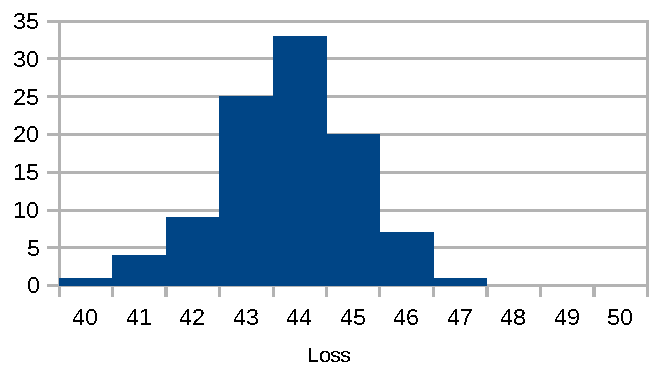
\includegraphics[width=0.31\textwidth]{figures/ablation/2-2}%
	}%
	\hspace*{\fill}
	\subfigure[Number of memory locations]{
		\label{fig:Raw_scatter}%
		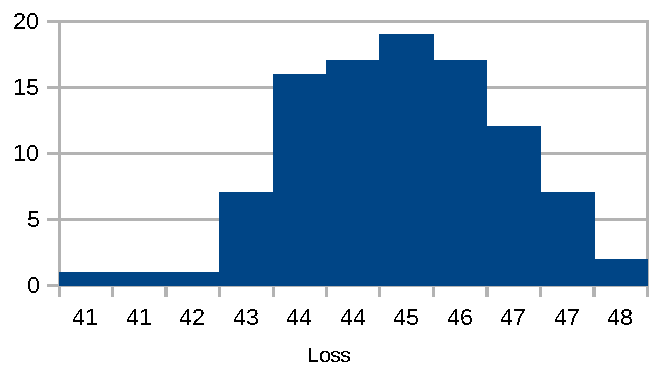
\includegraphics[width=0.31\textwidth]{figures/ablation/2-3}%
	}
	
	\subfigure[Baseline]{%
		\label{fig:Total_scatter}%
		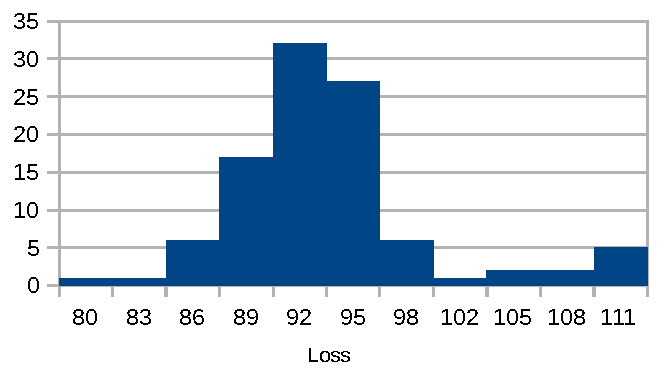
\includegraphics[width=0.31\textwidth]{figures/ablation/3-1}%
	}%
	\hspace*{\fill}
	\subfigure[Number of layers]{
		\label{fig:Num_scatter}%
		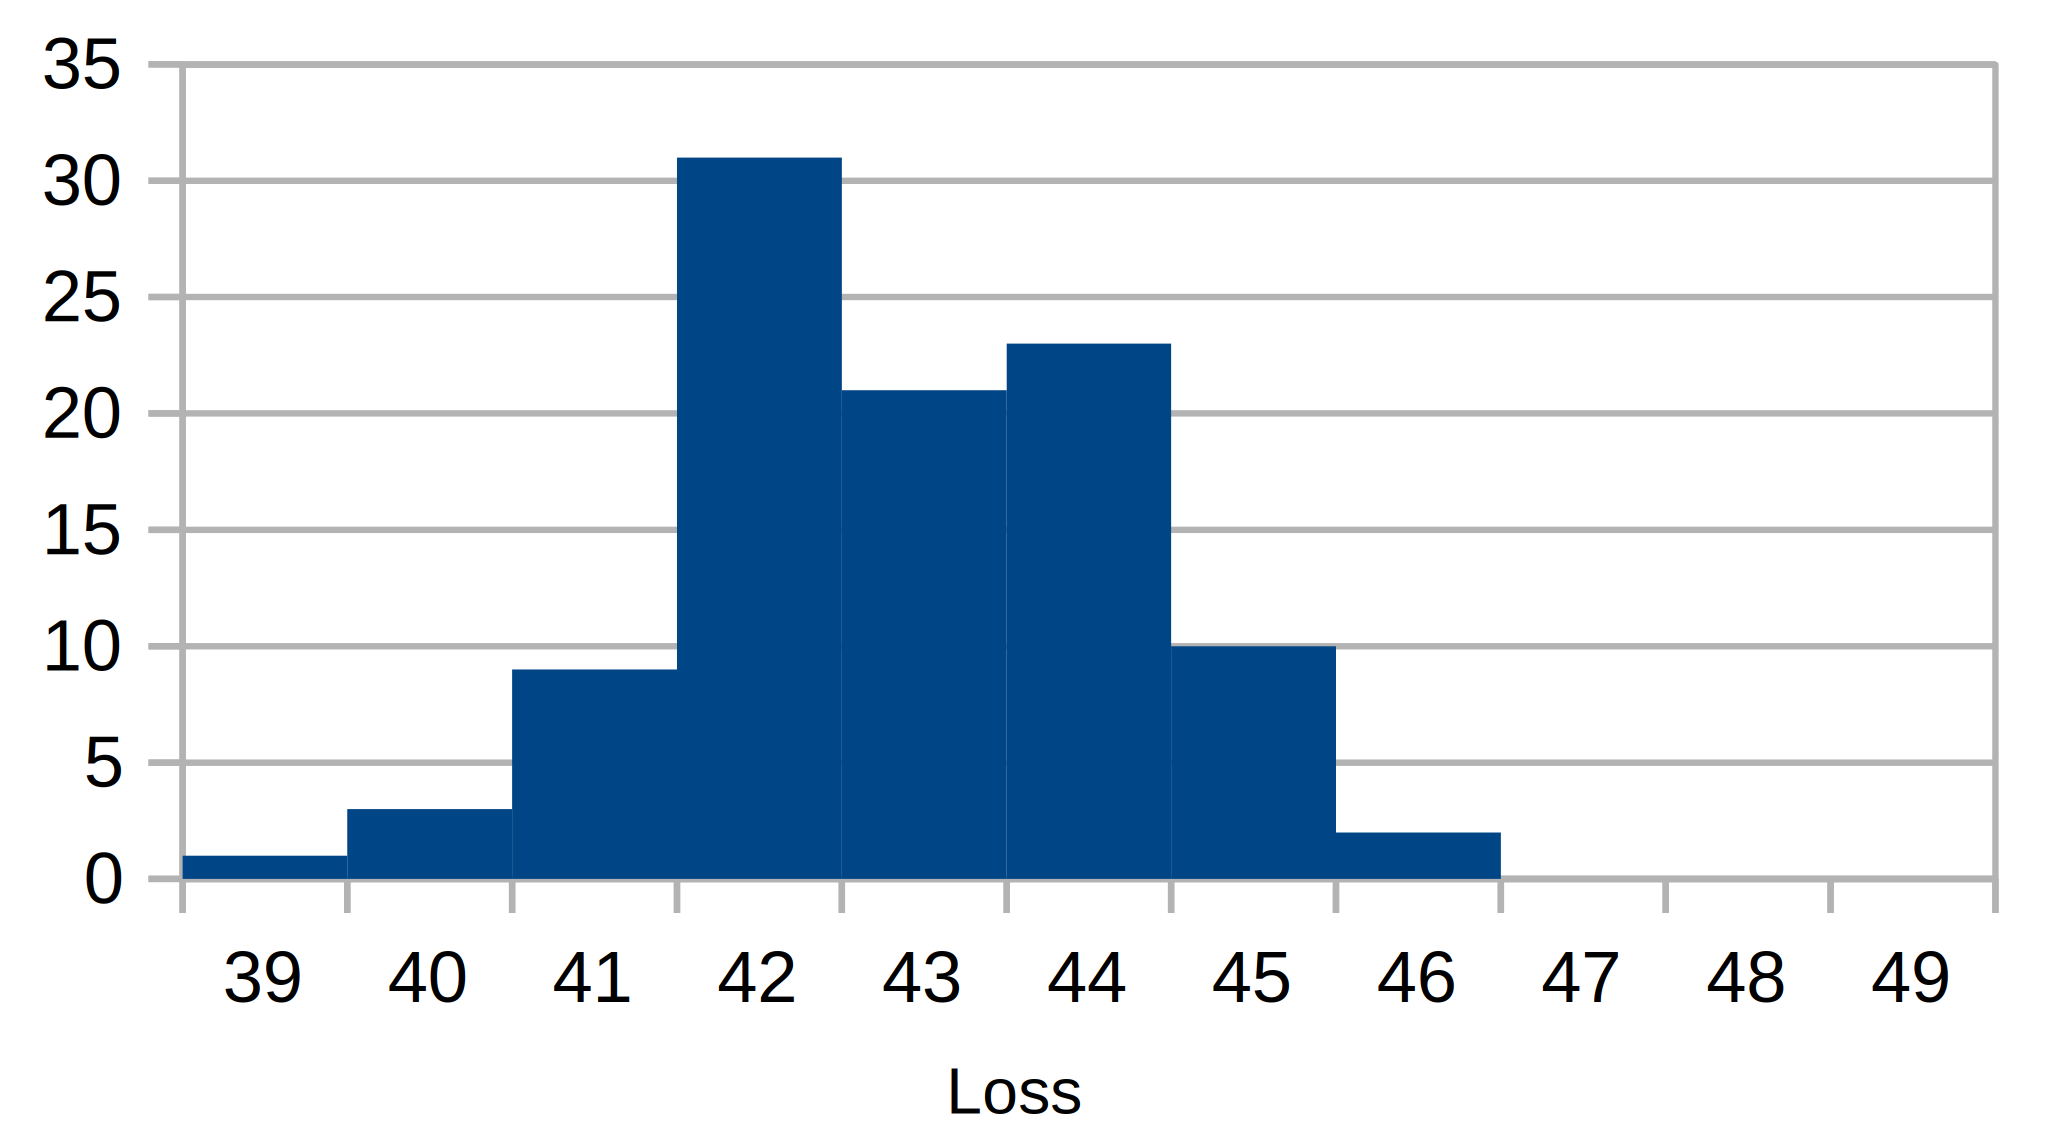
\includegraphics[width=0.31\textwidth]{figures/ablation/3-2}%
	}%
	\hspace*{\fill}
	\subfigure[Number of memory locations]{
		\label{fig:Raw_scatter}%
		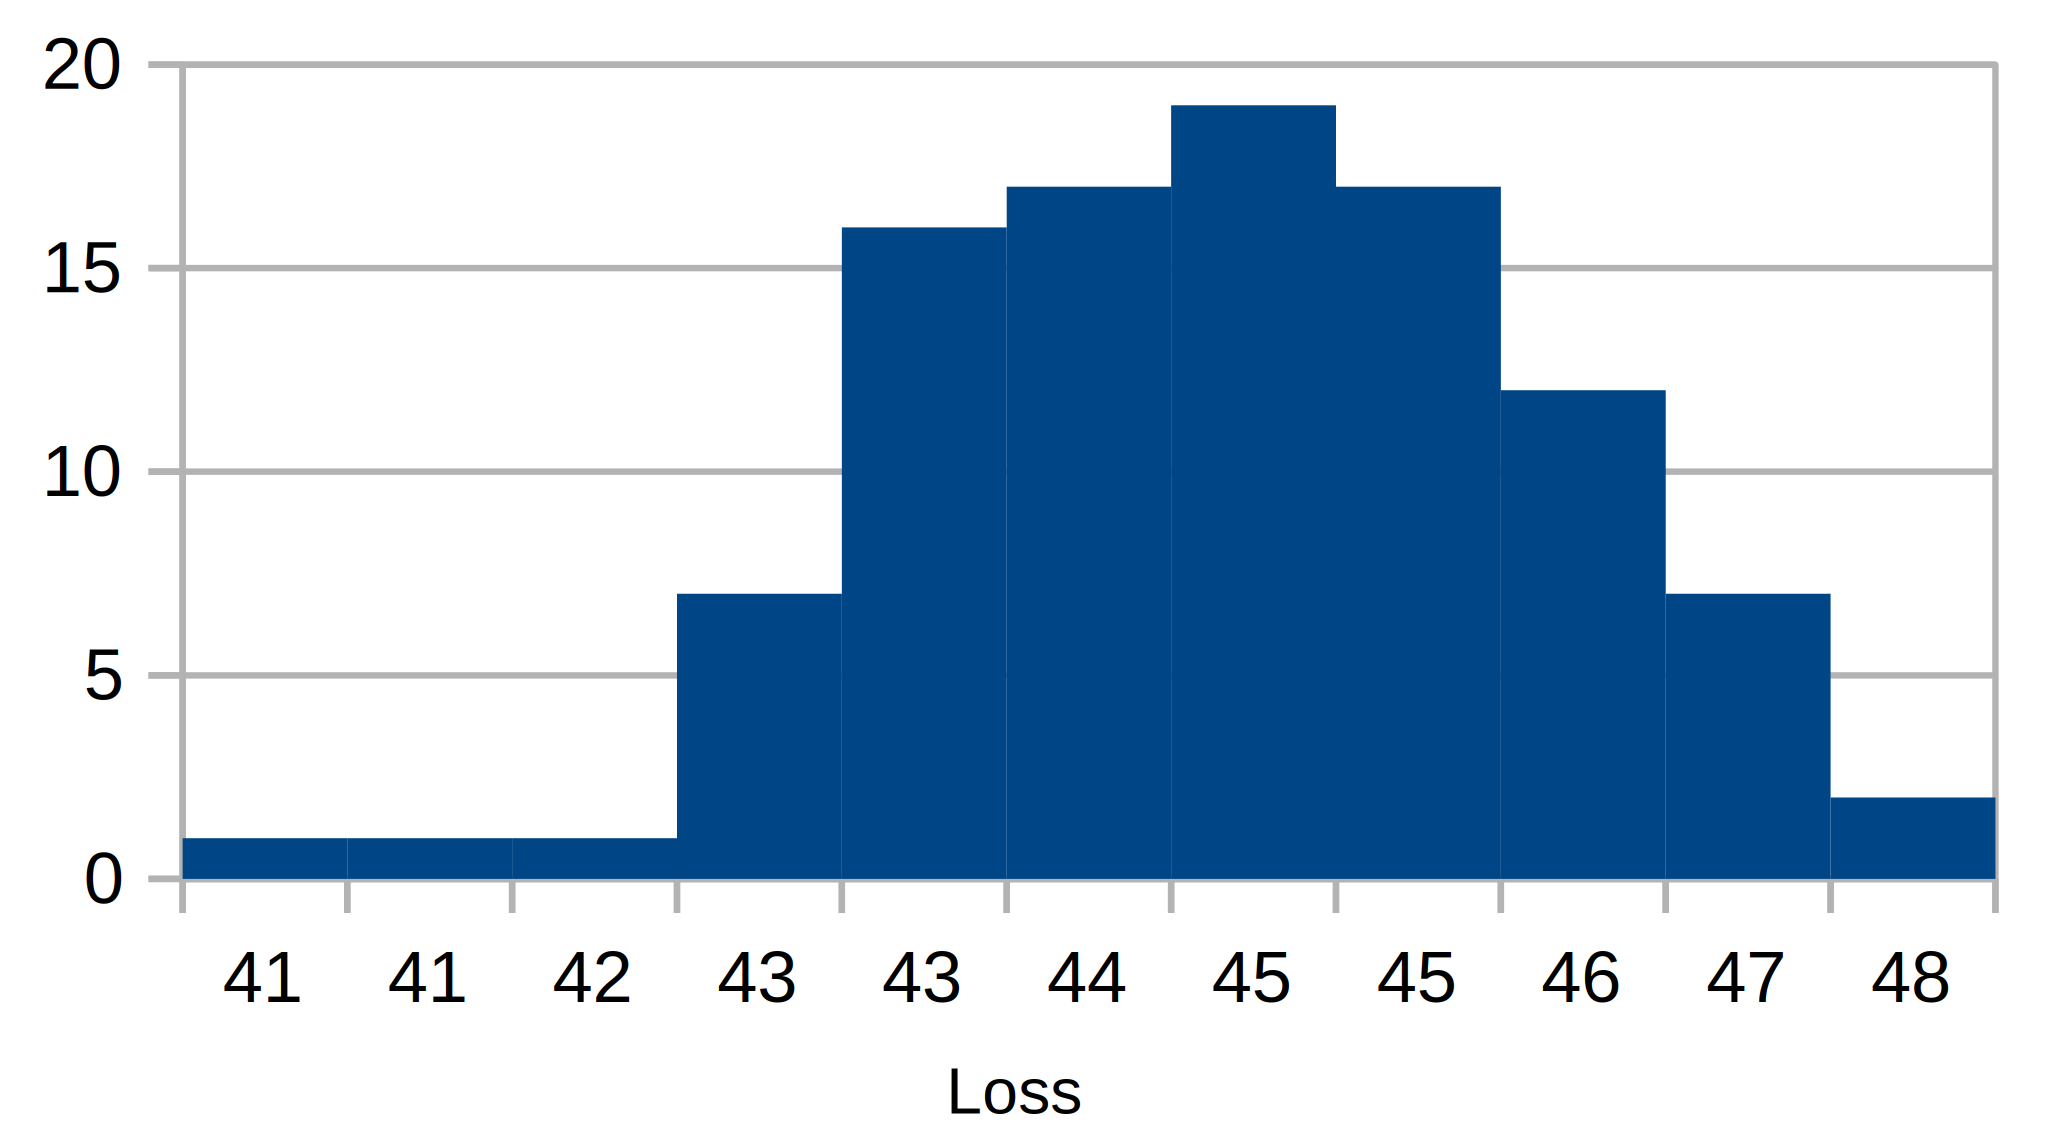
\includegraphics[width=0.31\textwidth]{figures/ablation/3-3}%
	}
	
	\subfigure[Baseline]{%
		\label{fig:Total_scatter}%
		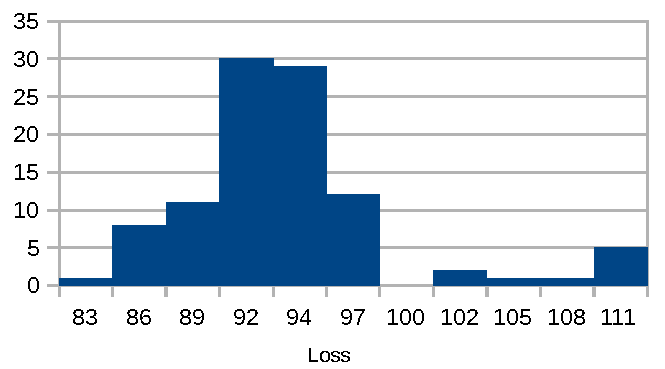
\includegraphics[width=0.31\textwidth]{figures/ablation/4-1}%
	}%
	\hspace*{\fill}
	\subfigure[Number of layers]{
		\label{fig:Num_scatter}%
		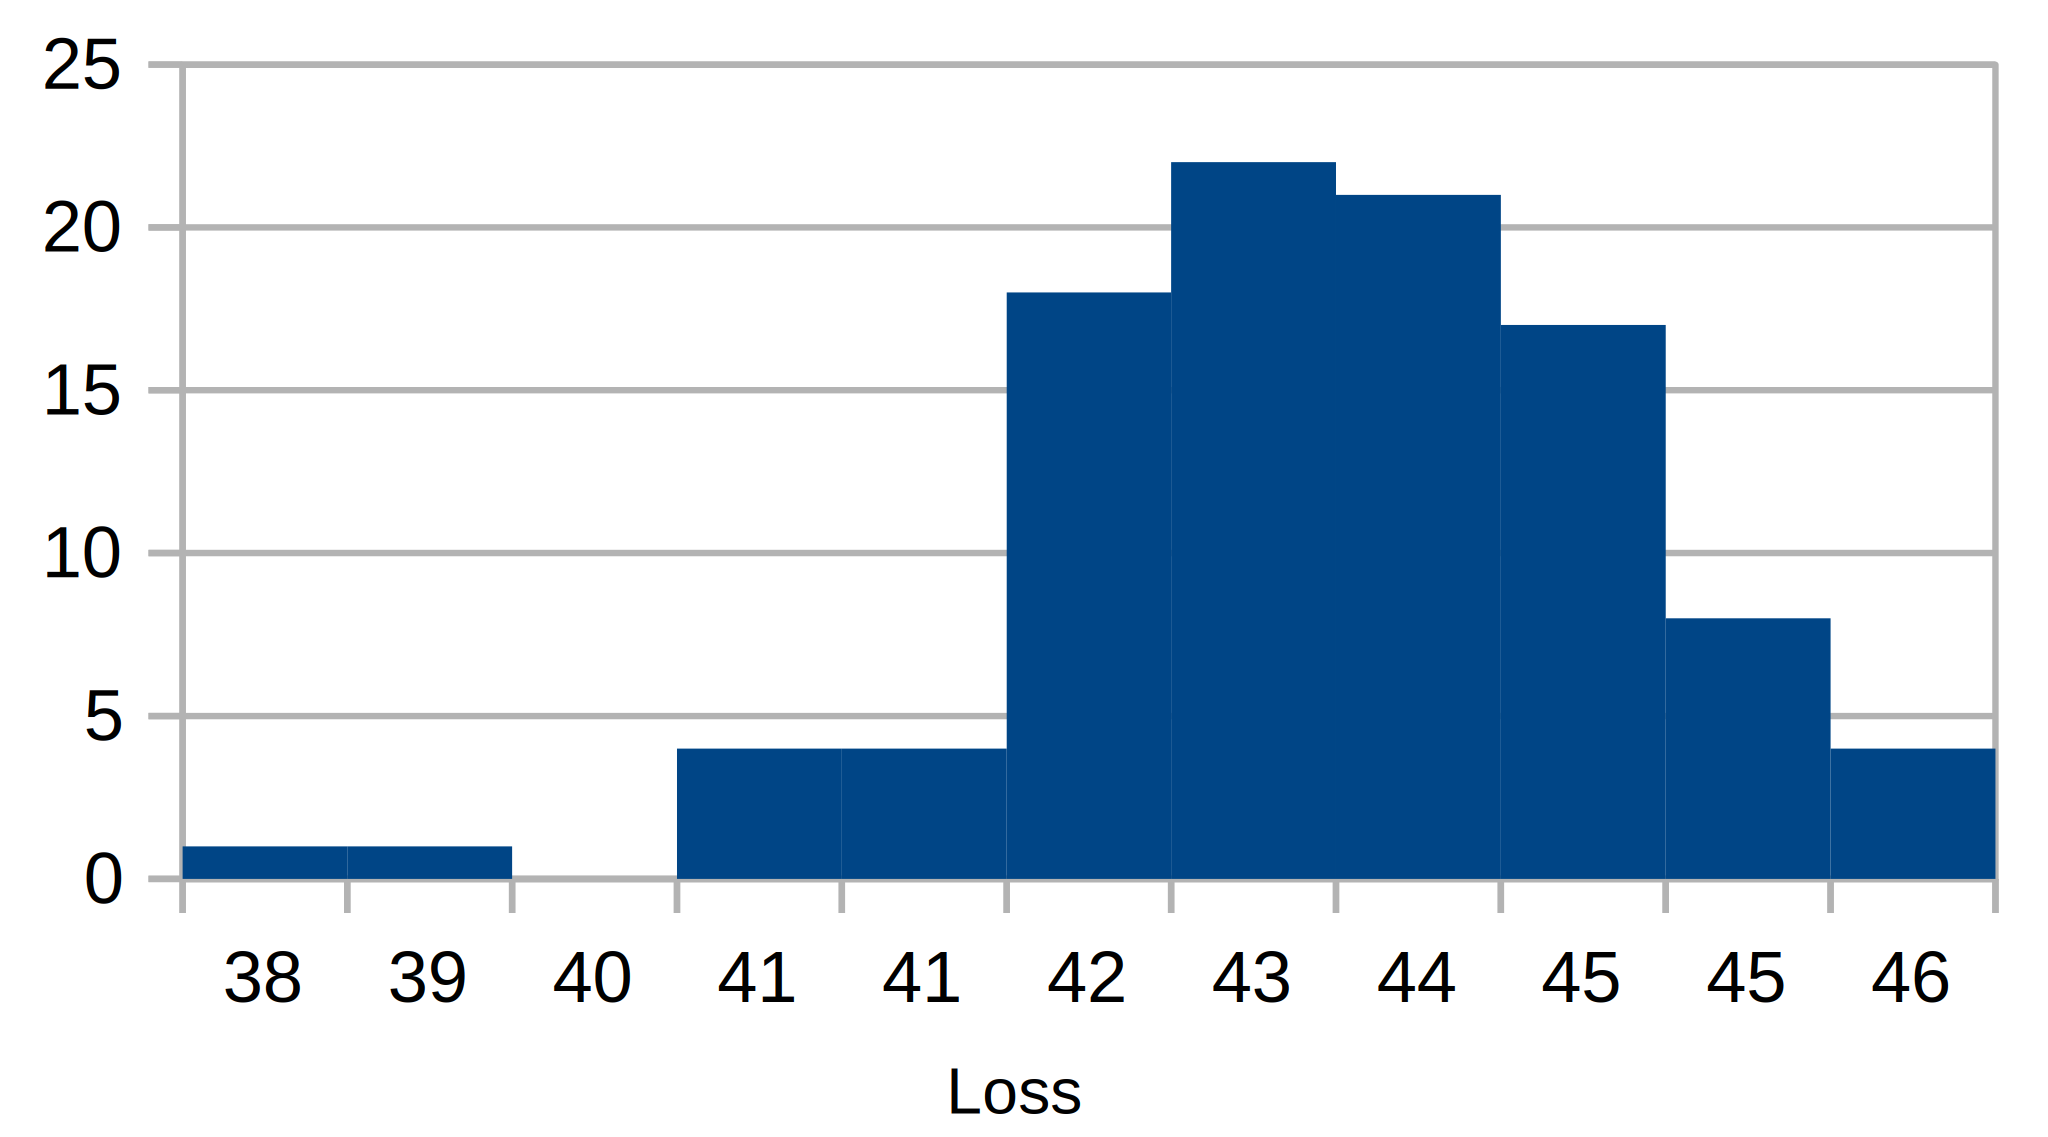
\includegraphics[width=0.31\textwidth]{figures/ablation/4-2}%
	}%
	\hspace*{\fill}
	\subfigure[Number of memory locations]{
		\label{fig:Raw_scatter}%
		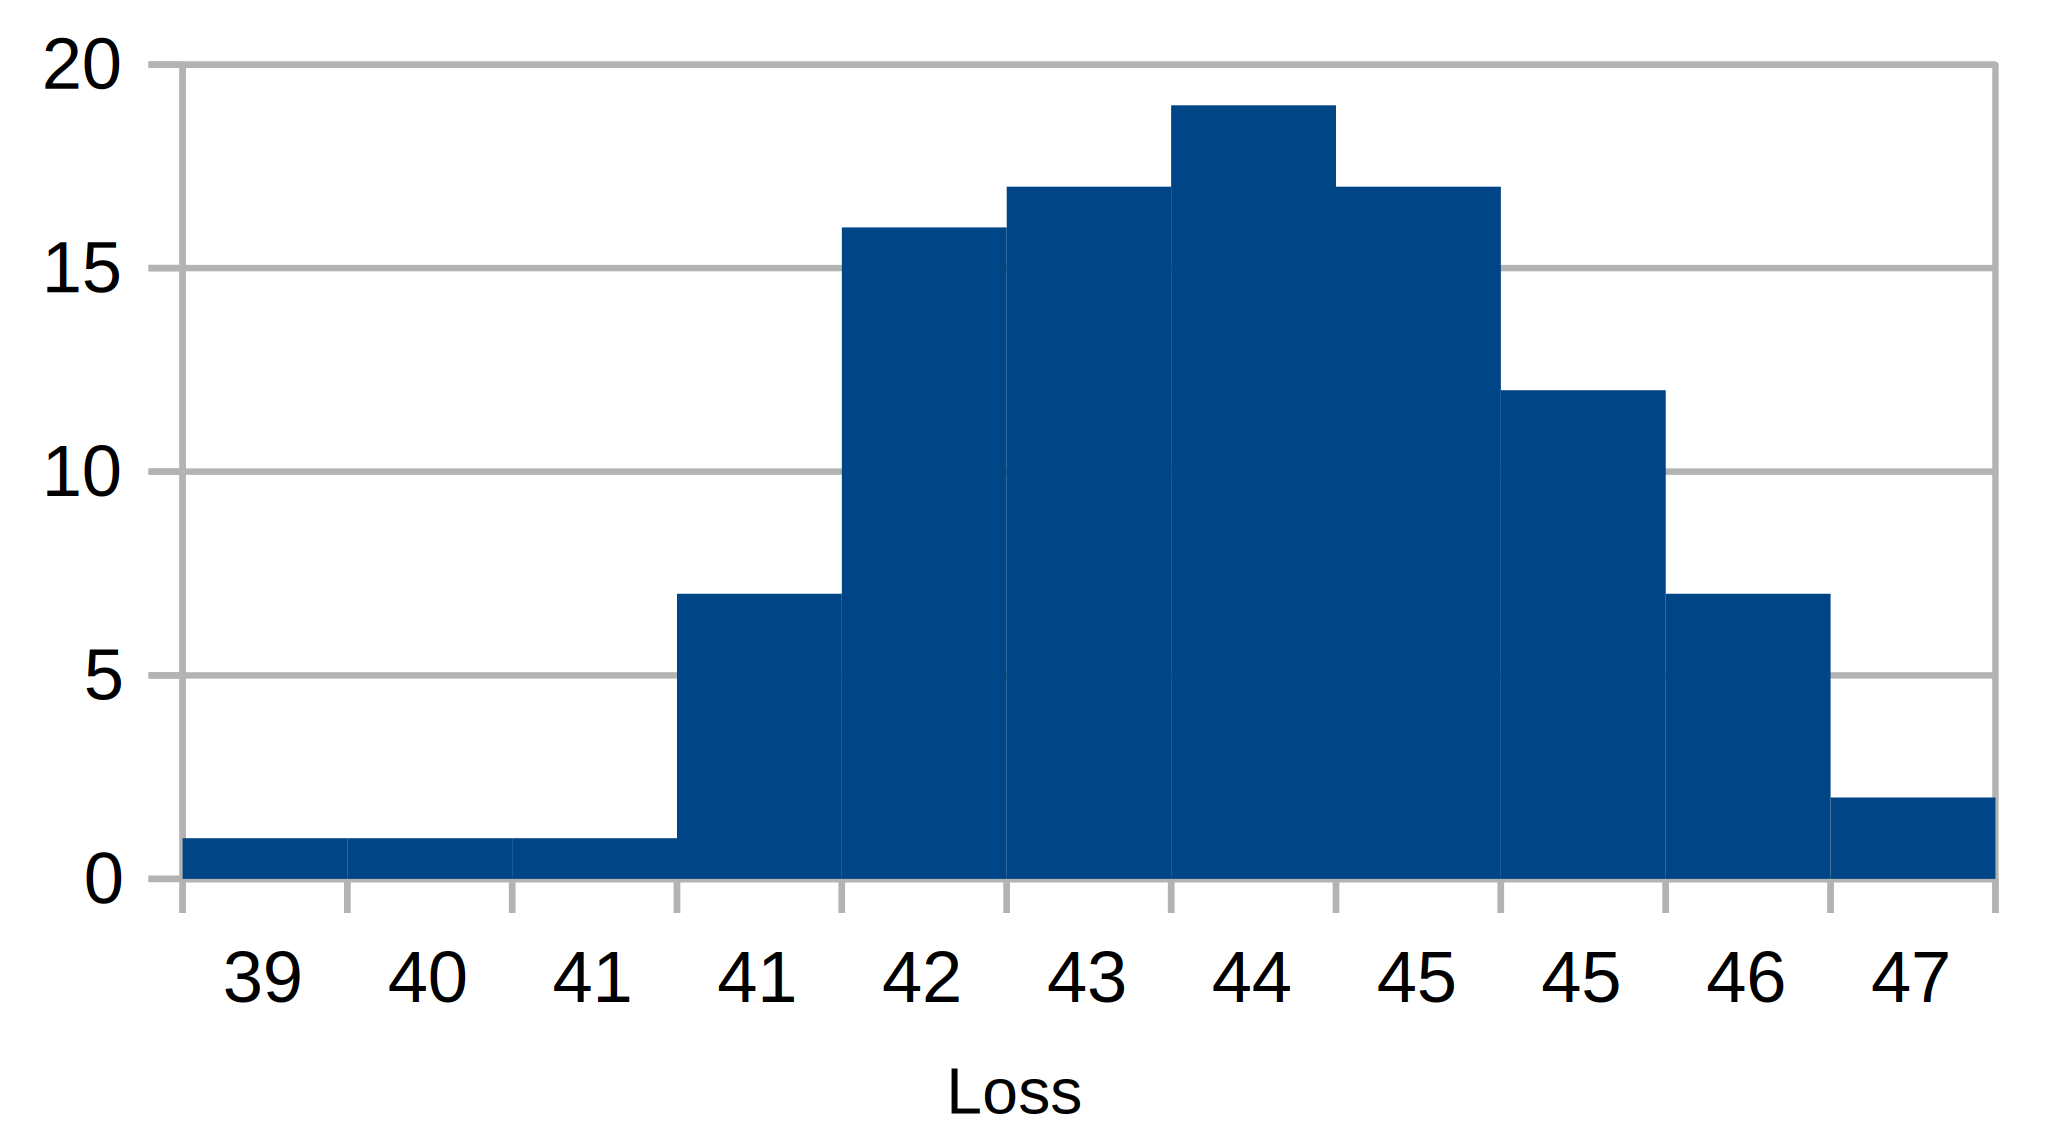
\includegraphics[width=0.31\textwidth]{figures/ablation/4-3}%
	}
	
	\subfigure[Baseline]{%
		\label{fig:Total_scatter}%
		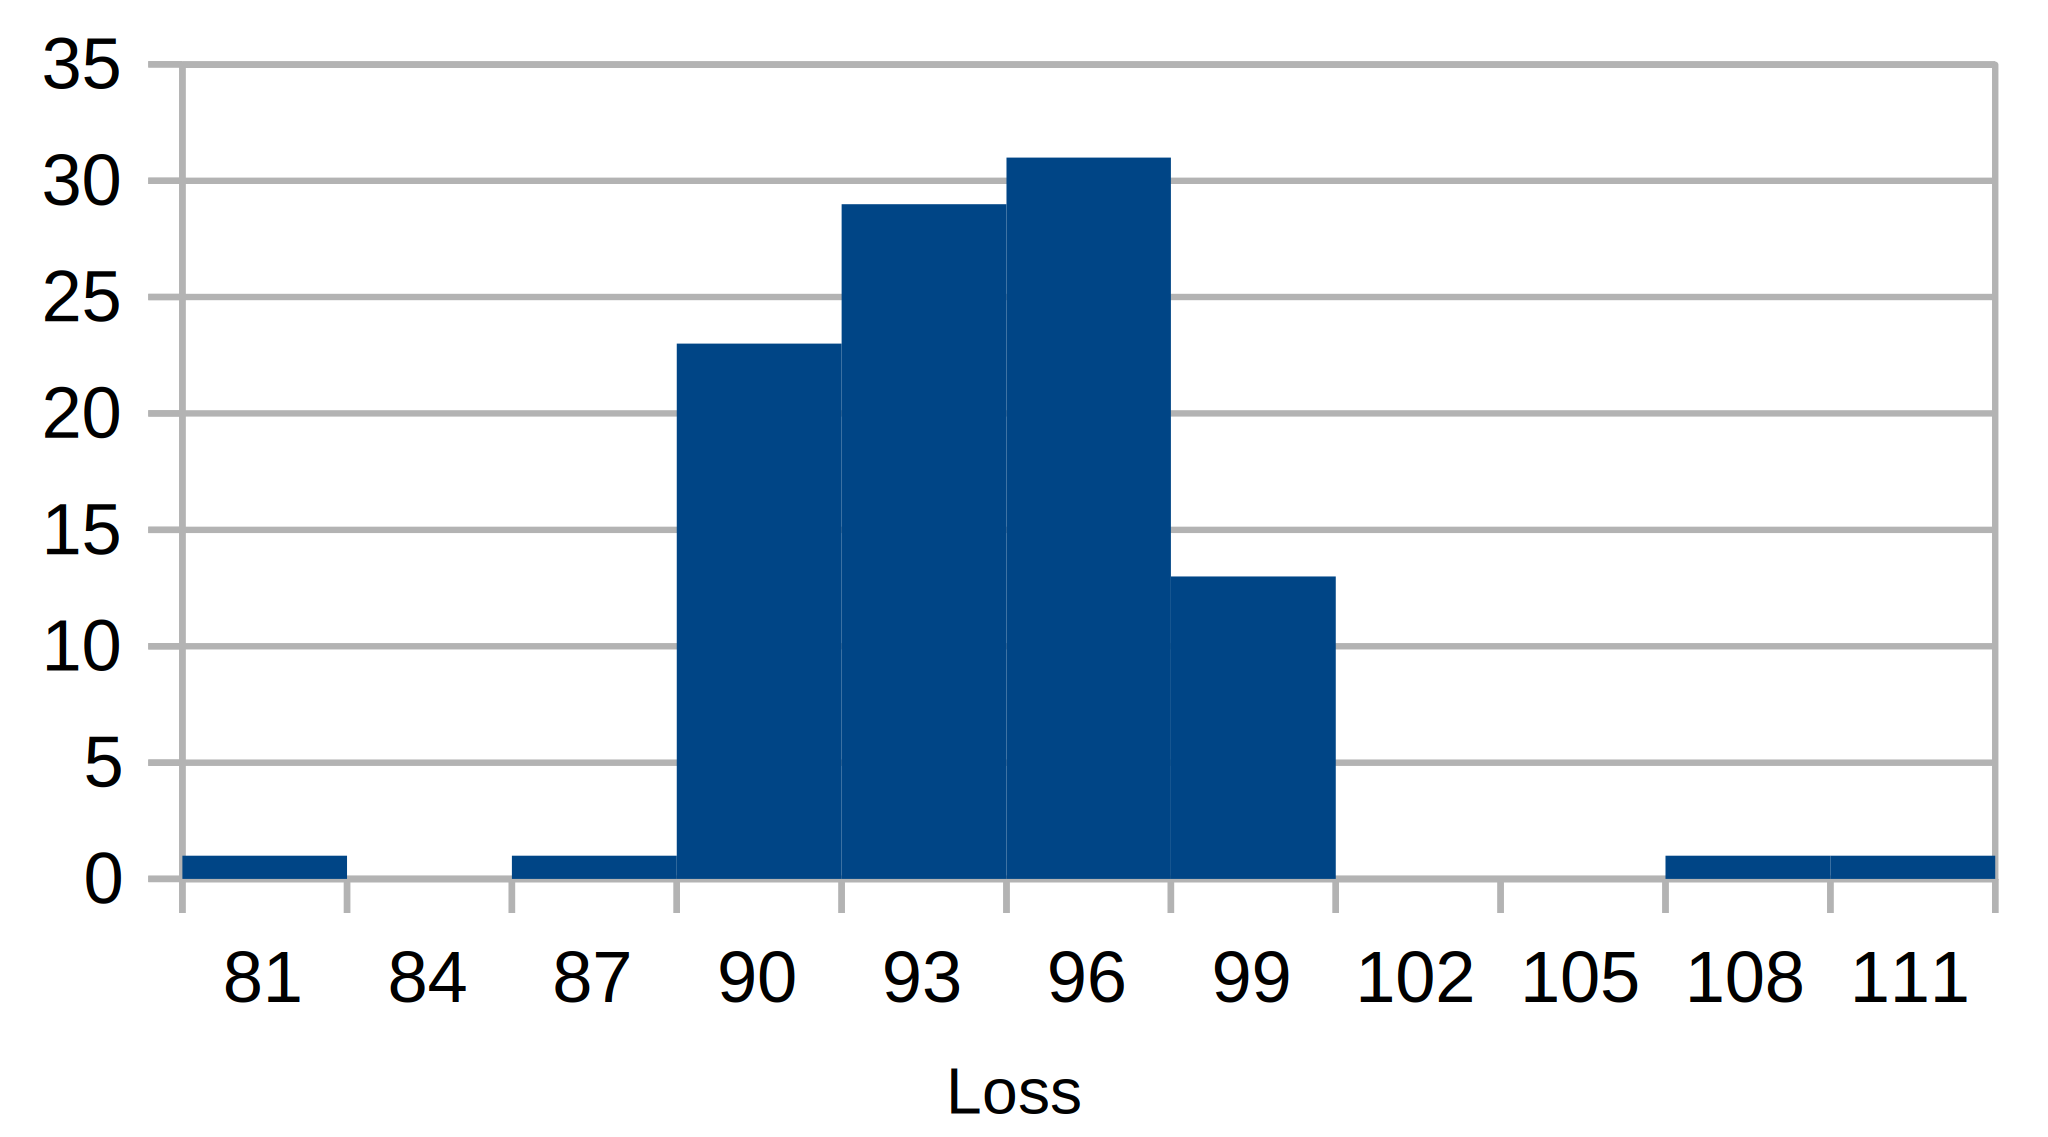
\includegraphics[width=0.31\textwidth]{figures/ablation/5-1}%
	}%
	\hspace*{\fill}
	\subfigure[Number of layers]{
		\label{fig:Num_scatter}%
		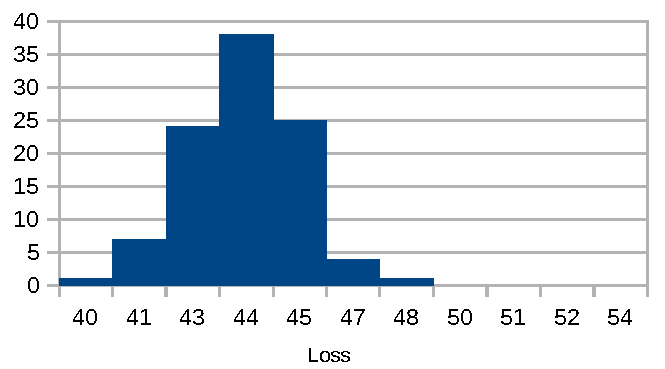
\includegraphics[width=0.31\textwidth]{figures/ablation/5-2}%
	}%
	\hspace*{\fill}
	\subfigure[Number of memory locations]{
		\label{fig:Raw_scatter}%
		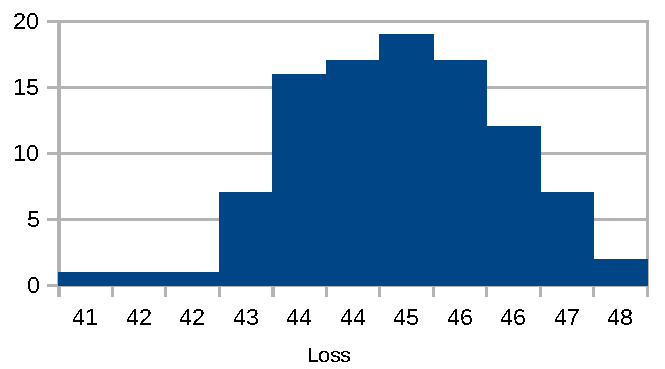
\includegraphics[width=0.31\textwidth]{figures/ablation/5-3}%
	}
	
	\subfigure[Baseline]{%
		\label{fig:Total_scatter}%
		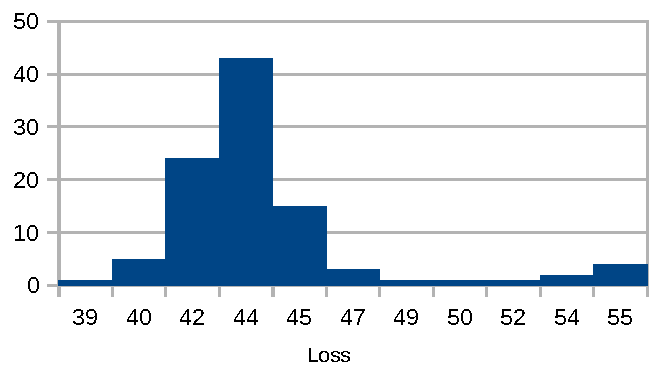
\includegraphics[width=0.31\textwidth]{figures/ablation/6-1}%
	}%
	\hspace*{\fill}
	\subfigure[Number of layers]{
		\label{fig:Num_scatter}%
		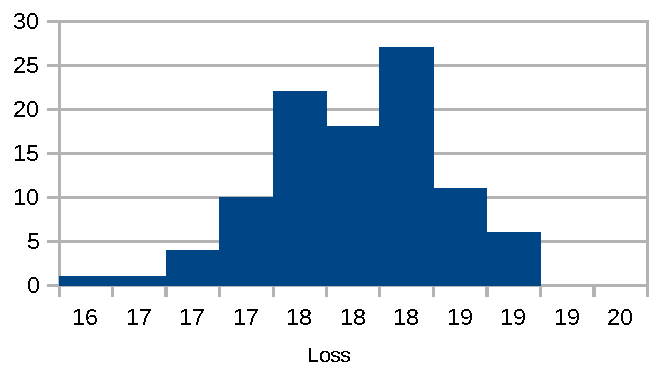
\includegraphics[width=0.31\textwidth]{figures/ablation/6-2}%
	}%
	\hspace*{\fill}
	\subfigure[Number of memory locations]{
		\label{fig:Raw_scatter}%
		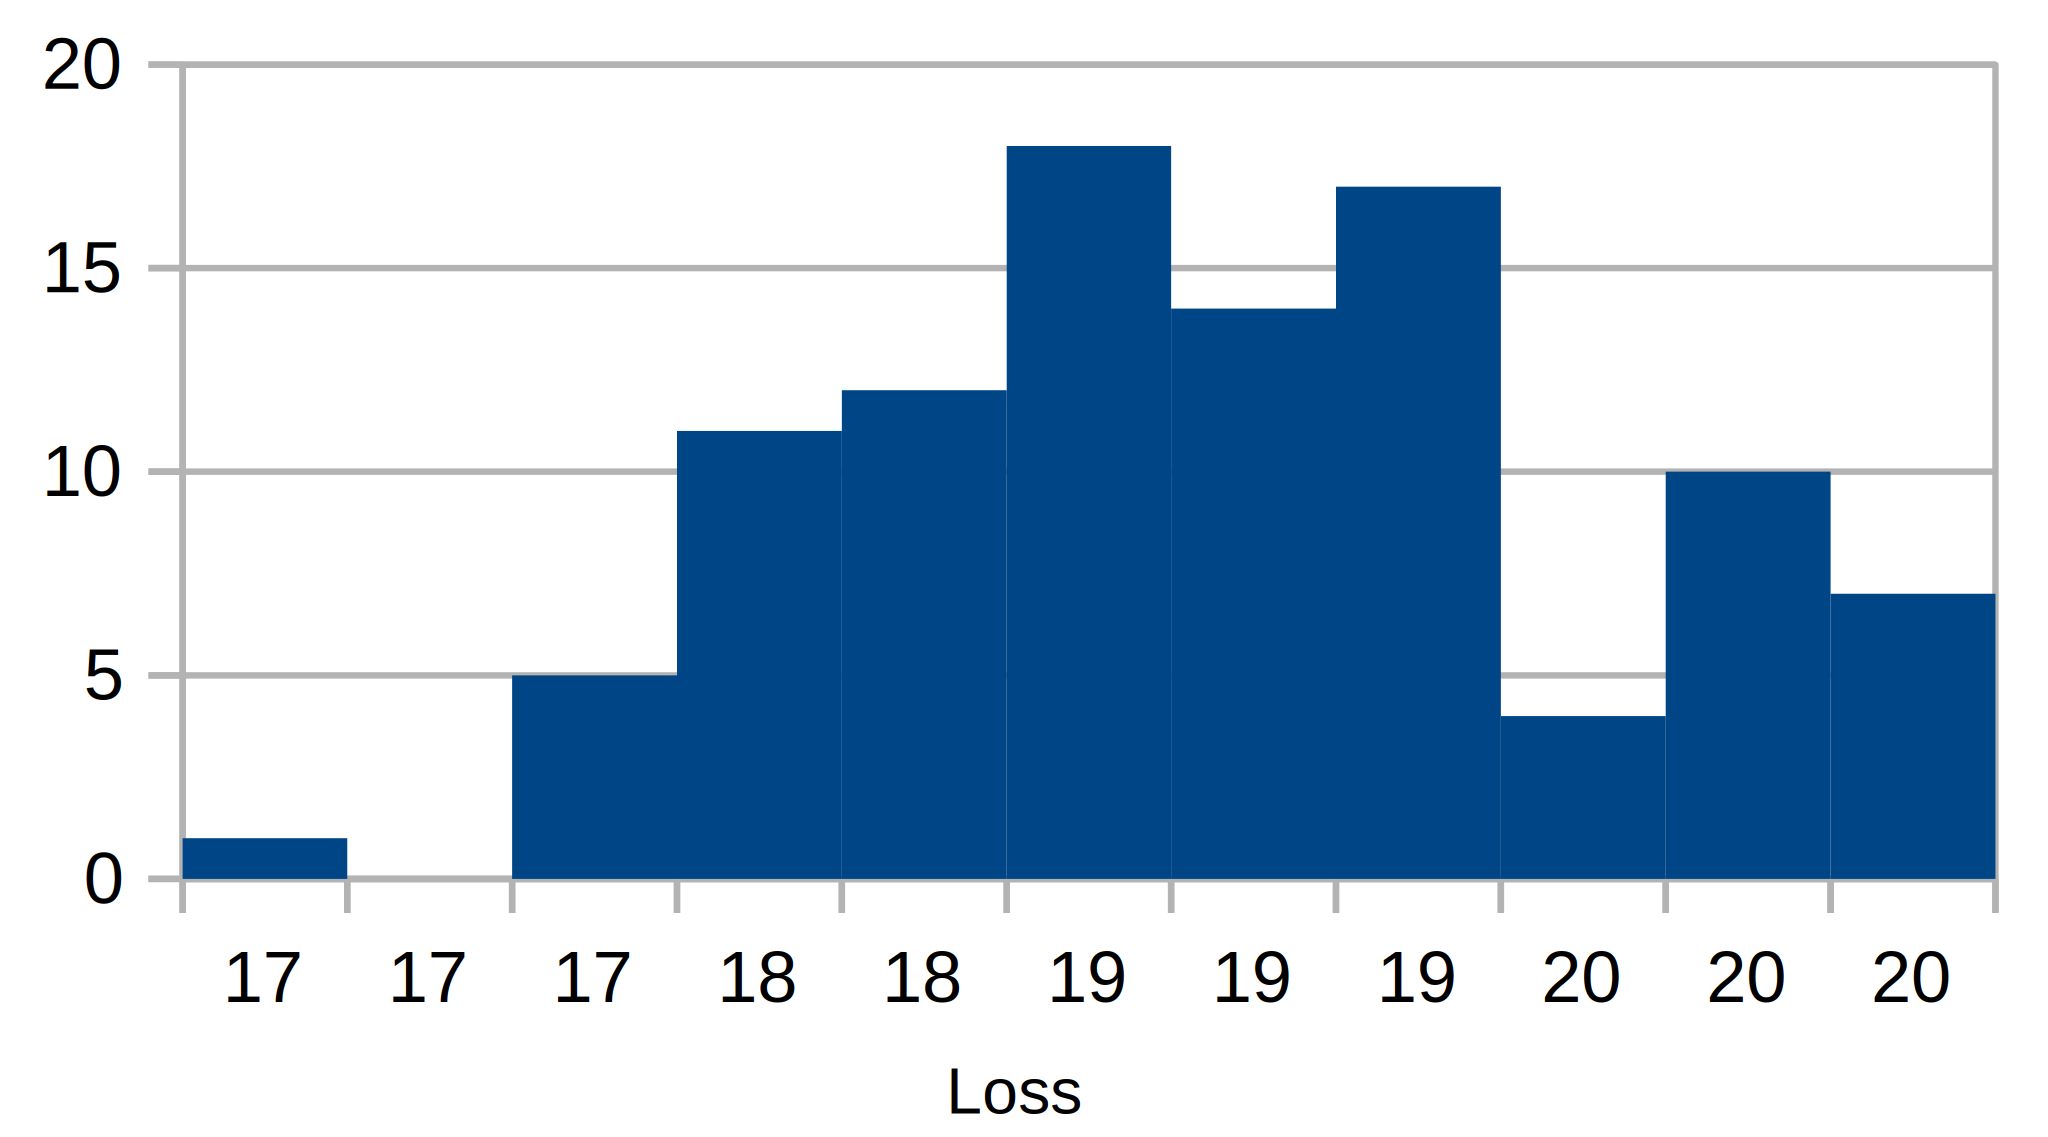
\includegraphics[width=0.31\textwidth]{figures/ablation/6-3}%
	}
	\caption{Learning curves for testing the model under different network parameters with same-sized data and different-sized data.}\label{fig:testing}
\end{figure*}